\documentclass[14pt, a4paper]{report}
\usepackage{fontspec}            % Must use XeLaTeX
\usepackage{amsmath}
% Toàn tài liệu chỉ dùng Times New Roman. Ký hiệu toán học dùng TeX Gyre Termes
% Math - bộ font toán được thiết kế tương thích với Times New Roman.
\setmainfont{Times New Roman}
\setsansfont{Times New Roman}
\setmonofont{Times New Roman}

\usepackage{unicode-math}
\setmathfont[Path=/usr/share/texmf-dist/fonts/opentype/public/tex-gyre-math/]{texgyretermes-math.otf}
\usepackage{fancyhdr}
\usepackage{tikzlings}
\usepackage{sectsty} % For coloring section headings
\usepackage{pdfpages}
\usepackage{epstopdf}
\usepackage{graphicx}
\usepackage{pifont}
\usepackage{booktabs}
\usepackage[
backend=biber,
style=numeric,
sorting=none
]{biblatex}

\addbibresource{references.bib}
\usepackage{placeins}
\setlength{\parskip}{10pt}
\usepackage{float}
\usepackage{multirow}
\usepackage{tabularx}
\usepackage{adjustbox}
\usepackage{listings}
\usepackage{xcolor}
\usepackage{algorithm}
\usepackage[noend]{algpseudocode}
\usepackage{siunitx}
\usepackage{subcaption}
\usepackage{indentfirst}
\setlength{\parindent}{1cm}
\setlength{\parskip}{0pt}
\setlength{\emergencystretch}{3em}
\usepackage[most]{tcolorbox}
\usepackage{enumerate}
\usepackage{tikz}
\tikzset{set/.style={draw,circle,inner sep=0pt,align=center}}
\usepackage{wasysym}
\usepackage{enumitem}
\usepackage{ragged2e}
\usepackage{etoolbox}

\usepackage[tikz]{bclogo}
\usepackage{longfbox}
\usepackage{pgfplots}
\usepackage{footnote}
\usepackage{fancyhdr}
\usepackage{babel}
\babelprovide[import, main]{vietnamese}
\usepackage[colorlinks=true, linkcolor=black, citecolor=black, urlcolor=blue]{hyperref}
\usepackage{setspace}
\usetikzlibrary {positioning,graphs,calc,decorations.pathmorphing,shapes,arrows.meta,arrows,shapes.misc,fit,patterns}
\usepgfplotslibrary{fillbetween}
\pgfplotsset{compat=1.9}
\usepackage[explicit]{titlesec}
\usepackage{lipsum}

% Define your colors
\definecolor{titlebgdark}{RGB}{0,163,243}
\definecolor{chapnumberbg}{RGB}{1,84,164}
\definecolor{chapname}{RGB}{1,84,164}

\rhead{\color{gray}\textbf{ \leftmark}}
\lhead{\color{chapname}\textbf{Nhóm 5 - CS106 - Trí tuệ nhân tạo}}

\usepackage{tikzpagenodes}
\usepackage[top=2.5cm, bottom=2.5cm, left=3cm, right=2cm]{geometry}
\usepackage{longtable}
\usepackage{tabularx}
\usepackage{array}
\usepackage{pdfpages}
\usetikzlibrary{fit}
\urlstyle{same}

% Apply color to section and subsection headings
\sectionfont{\color{chapname}\normalfont\bfseries\large}
\subsectionfont{\color{chapname}\normalfont\bfseries\large}

\titleformat{\chapter}[display]
{\Large}
{}
{0pt}
{%
    \begin{tikzpicture}
        \node[
        draw=chapname,
        rounded corners,
        outer sep=0pt,
        inner sep=6pt,
        rotate=90,
        line width=1pt,
        font=\Large\color{chapnumberbg}\bfseries
        ]
        (chapname)
        {\chaptertitlename};
        \node[
        fill=chapnumberbg,
        minimum width=2cm,
        minimum height=2.3cm,
        rounded corners,
        anchor=west,
        font=\color{white}\fontsize{40}{48}\selectfont\bfseries
        ]
        at ([xshift=6pt]chapname.south)
        (chapnumber)
        {\thechapter};
        \node[
        anchor=west,
        text width=\textwidth-4cm,
        font=\bfseries\LARGE
        ]
        at ([xshift=10pt]chapnumber.east)
        {#1};
        \fill[
        overlay,
        draw=none,
        line width=0pt,
        rounded corners=1pt,
        left color=chapnumberbg,
        right color=chapnumberbg!10
        ]
        ([yshift=-3pt]chapname.north west) rectangle ++(\textwidth,-3pt);
    \end{tikzpicture}%
}
\titleformat{name=\chapter,numberless}[display]
{\normalfont}
{}
{0pt}
{%
    \begin{tikzpicture}
        \node[
        anchor=west,
        inner sep=0pt,
        outer sep=0pt,
        text width=\textwidth,
        font=\bfseries\LARGE
        ]
        (chaptitle)
        {#1};
        \fill[
        overlay,
        draw=none,
        line width=0pt,
        rounded corners=1pt,
        left color=chapnumberbg,
        right color=chapnumberbg!10
        ]
        ([yshift=-3pt]chaptitle.south west) rectangle ++(\textwidth,-3pt);
    \end{tikzpicture}%
}
\titlespacing{\chapter}{0pt}{-40pt}{1cm}

\begin{document}
\begin{spacing}{1.5}
\pagestyle{fancy}

\includepdf[]{cover.pdf}
\setcounter{tocdepth}{1}
\large

\thispagestyle{empty}
\begin{justify}

\tableofcontents
\thispagestyle{empty}
\clearpage

\chapter{GIỚI THIỆU}
\setcounter{page}{1}
\section{Đặt vấn đề}
Sự phát triển nhanh chóng của các hình thức thanh toán điện tử và thẻ tín dụng giúp việc giao dịch trở nên thuận tiện, nhưng đồng thời cũng kéo theo nguy cơ gian lận ngày càng gia tăng. Các giao dịch gian lận gây thiệt hại lớn cho ngân hàng, đơn vị thanh toán và chính khách hàng \cite{bhattacharyya2011creditcard}, do đó việc phát hiện kịp thời các giao dịch bất thường là một bài toán quan trọng trong lĩnh vực tài chính.

Đặc điểm nổi bật của bài toán phát hiện gian lận là dữ liệu thường mất cân bằng nghiêm trọng: số giao dịch gian lận chỉ chiếm một tỷ lệ rất nhỏ so với giao dịch bình thường \cite{he2009imbalanced, dalpozzolo2015credit}. Một mô hình đơn giản dự đoán tất cả giao dịch là hợp lệ vẫn có thể đạt Accuracy rất cao nhưng hoàn toàn bỏ sót gian lận. Vì vậy, bài toán cần được đánh giá bằng các chỉ số phù hợp như Recall, F2-Score hay PR-AUC thay vì chỉ dựa vào Accuracy \cite{davis2006pr}.

Trong khuôn khổ môn học Trí tuệ nhân tạo, đề tài xây dựng một hệ thống học máy có khả năng phân loại một giao dịch tài chính thành hai nhóm: giao dịch hợp lệ (nhãn 0) và giao dịch gian lận (nhãn 1). Toàn bộ quy trình từ nạp dữ liệu, làm sạch, phân tích khám phá, tạo đặc trưng, xây dựng và đánh giá mô hình được thực hiện một cách bài bản trên cùng một bộ dữ liệu mô phỏng giao dịch thẻ tín dụng.

\section{Mục tiêu của đề tài}
Đề tài hướng tới các mục tiêu chính sau đây:
\begin{itemize}
    \item Xây dựng quy trình xử lý hoàn chỉnh cho dữ liệu giao dịch thẻ tín dụng: nạp dữ liệu, làm sạch, xử lý dữ liệu thiếu, tạo đặc trưng và chuẩn hóa dữ liệu.
    \item Phân tích khám phá dữ liệu nhằm nhận diện các đặc điểm của giao dịch gian lận như loại hình dịch vụ có rủi ro cao, giá trị bất thường của số tiền giao dịch.
    \item Xây dựng và huấn luyện năm thuật toán phân loại: Random Forest, XGBoost (hai cấu hình), LightGBM và CatBoost, kết hợp các kỹ thuật xử lý dữ liệu mất cân bằng như \texttt{class\_weight}, \texttt{scale\_pos\_weight}, \texttt{auto\_class\_weights} và SMOTE nhẹ; sau đó tích hợp các mô hình tốt nhất bằng kỹ thuật xếp chồng \texttt{StackingClassifier}.
    \item Thiết kế sáu thử nghiệm có kiểm soát để đánh giá ảnh hưởng của phương pháp biểu diễn đặc trưng (đặc trưng gốc, \texttt{OneHotEncoder}, \texttt{TargetEncoder}) và của việc loại bỏ các đặc trưng chứa nhiễu, trong khi giữ nguyên quy trình chia tập và tinh chỉnh siêu tham số.
    \item Đánh giá và so sánh hiệu suất các mô hình dựa trên các chỉ số Precision, Recall, F1-Score, F2-Score, ROC-AUC, PR-AUC, FNR và FPR; lựa chọn mô hình đề xuất cuối cùng.
\end{itemize}

\section{Phạm vi phân tích}
Bộ dữ liệu của đề tài gồm 30\,058 giao dịch thẻ tín dụng mô phỏng được ghi nhận trong giai đoạn từ ngày 21/06 đến ngày 30/06/2020, với 23 cột thuộc tính mô tả thời gian giao dịch, thẻ, đơn vị chấp nhận thanh toán, loại hình dịch vụ, số tiền, vị trí địa lý và nhãn gian lận. Trong đó có 29\,925 giao dịch hợp lệ và 133 giao dịch gian lận, khiến lớp gian lận nhỏ hơn lớp hợp lệ 225 lần.

Đề tài tập trung vào việc xây dựng và so sánh năm thuật toán Random Forest, XGBoost, LightGBM, CatBoost và mô hình xếp chồng Stacking trên cùng một bộ dữ liệu, cùng bốn chiến lược xử lý mất cân bằng lớp (điều chỉnh trọng số lớp, gán trọng số cho lớp thiểu số, trọng số tự động cân bằng và sinh dữ liệu tổng hợp SMOTE nhẹ). Các vấn đề về triển khai hệ thống phát hiện gian lận theo thời gian thực hay tích hợp nghiệp vụ ngân hàng không thuộc phạm vi nghiên cứu của đồ án.

\chapter{PHƯƠNG PHÁP THU THẬP VÀ TIỀN XỬ LÝ DỮ LIỆU}
\section{Thu thập dữ liệu giao dịch}
Bộ dữ liệu được sử dụng trong đồ án là tập dữ liệu giao dịch thẻ tín dụng mô phỏng, gồm 30\,058 giao dịch và 23 cột thuộc tính. Dữ liệu được lưu trữ trên Google Sheets và được nạp trực tiếp vào chương trình bằng thư viện \texttt{pandas} \cite{mckinney2010pandas} dưới dạng CSV. Quá trình nạp dữ liệu và làm sạch dữ liệu lần lượt được trình bày trong Hình \ref{fig:code_loading} và Hình \ref{fig:code_cleaning}.

\begin{figure}[H]
    \centering
    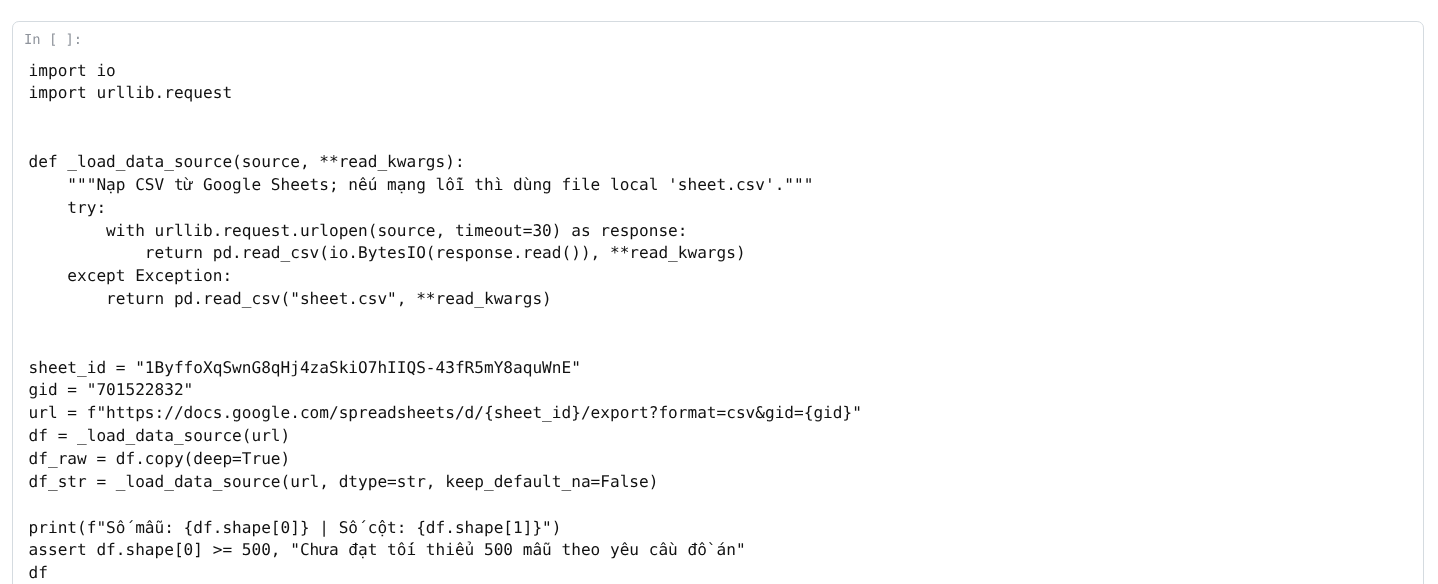
\includegraphics[width=\linewidth,height=0.9\textheight,keepaspectratio]{figures/code_cleaning_1.png}
    \caption{Đoạn chương trình nạp dữ liệu từ Google Sheets}
    \label{fig:code_loading}
\end{figure}

\begin{figure}[htbp]
    \centering
    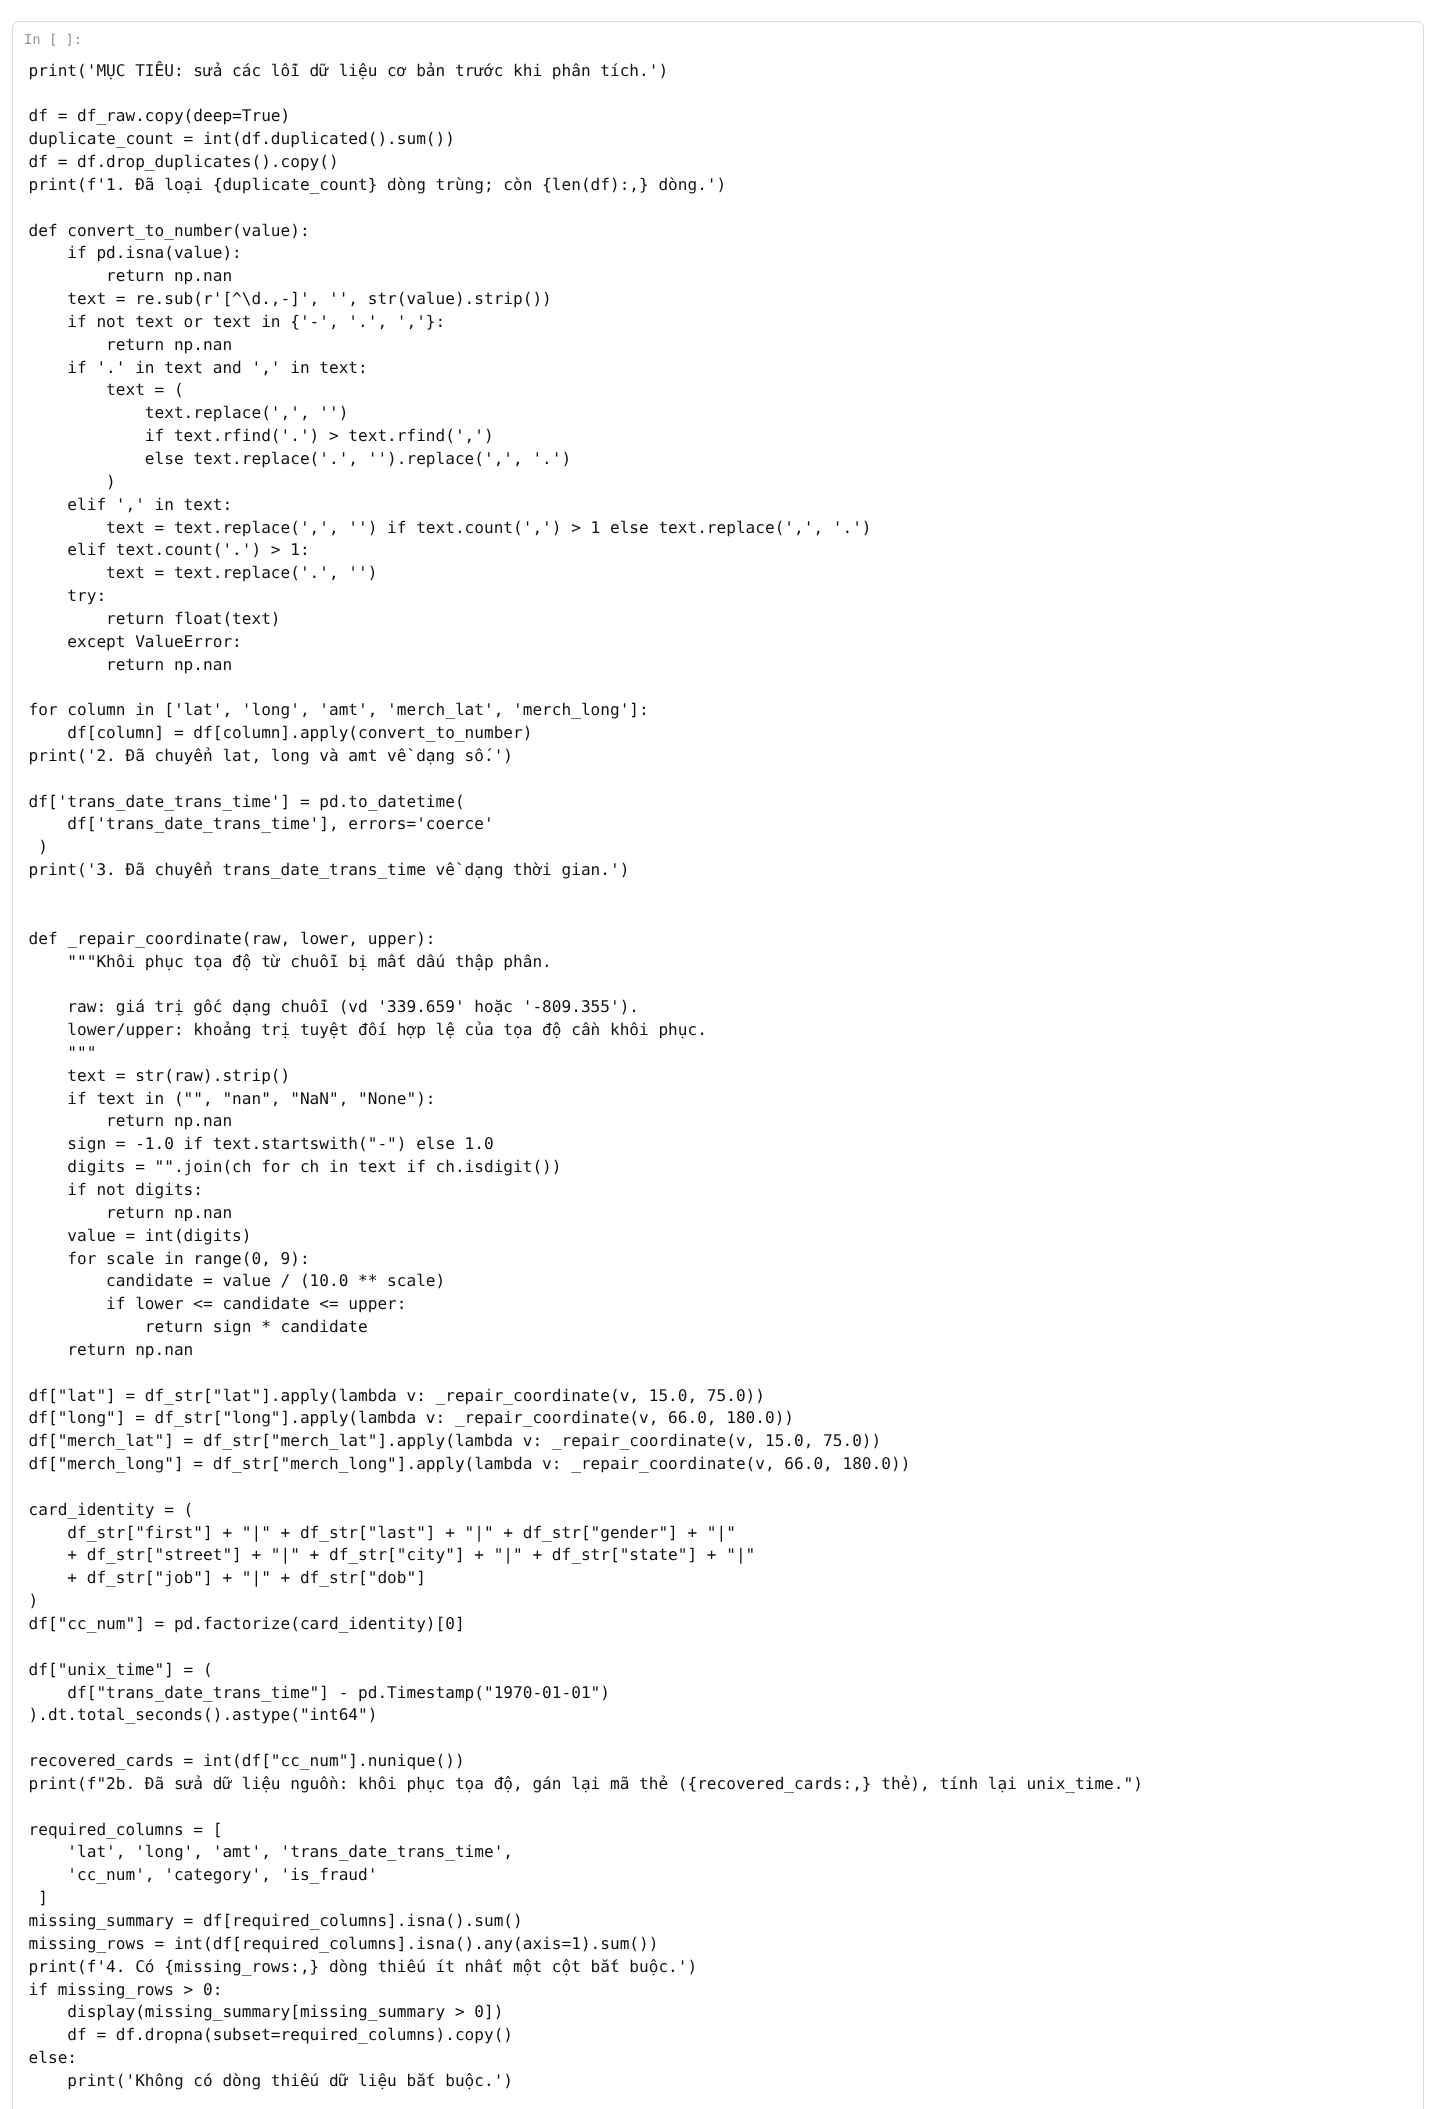
\includegraphics[width=\linewidth,height=0.9\textheight,keepaspectratio]{figures/code_cleaning_2.png}
    \caption{Đoạn chương trình làm sạch dữ liệu}
    \label{fig:code_cleaning}
\end{figure}

\section{Mô tả bộ dữ liệu}
Bộ dữ liệu mô tả hoạt động giao dịch của 909 thẻ tín dụng tại 693 điểm chấp nhận thanh toán thuộc 50 bang của Hoa Kỳ, trong khoảng thời gian 10 ngày, từ ngày 21/06 đến ngày 30/06/2020. Mỗi bản ghi tương ứng với một giao dịch. Số tiền giao dịch dao động từ 1\,USD đến 6\,600{,}44\,USD, với trung vị 46{,}28\,USD. Bảng \ref{tab:data_fields} liệt kê chi tiết các cột quan trọng của bộ dữ liệu.

\begin{table}[H]
\centering
\fontsize{11}{13.6}\selectfont
\renewcommand{\arraystretch}{1.2}
\setlength{\tabcolsep}{6pt}
\begin{tabularx}{\textwidth}{|p{4.2cm}|p{2.2cm}|X|}
\hline
\textbf{Đặc trưng} & \textbf{Kiểu dữ liệu} & \textbf{Mô tả} \\
\hline
trans\_date\_trans\_time & datetime & Thời điểm giao dịch \\
\hline
cc\_num & string & Mã thẻ tín dụng \\
\hline
merchant & string & Đơn vị chấp nhận thanh toán \\
\hline
category & string & Loại hình dịch vụ như mua sắm, ăn uống, du lịch \\
\hline
amt & float & Số tiền giao dịch (USD) \\
\hline
gender & string & Giới tính chủ thẻ \\
\hline
city / state & string & Thành phố / bang nơi giao dịch \\
\hline
lat / long & float & Vĩ độ / kinh độ vị trí thường trú của chủ thẻ \\
\hline
city\_pop & int & Dân số thành phố \\
\hline
job / dob & string & Nghề nghiệp / ngày sinh chủ thẻ \\
\hline
trans\_num / unix\_time & string & Mã giao dịch / thời gian dạng epoch \\
\hline
merch\_lat / merch\_long & float & Vị trí của đơn vị chấp nhận thanh toán \\
\hline
is\_fraud & int & Nhãn: 0 = hợp lệ, 1 = gian lận \\
\hline
\end{tabularx}
\caption{Các đặc trưng của bộ dữ liệu}
\label{tab:data_fields}
\end{table}

Phân bố nhãn của bộ dữ liệu cho thấy tính mất cân bằng nghiêm trọng: có 29\,925 giao dịch hợp lệ nhưng chỉ có 133 giao dịch gian lận, tương ứng tỷ lệ gian lận 0{,}44\%. Lớp lớn gấp 225 lần lớp nhỏ. Vì vậy, Accuracy không phản ánh đúng khả năng phát hiện gian lận của mô hình và không được dùng làm tiêu chí đánh giá chính trong đồ án.

\section{Tiền xử lý dữ liệu}
\subsection{Làm sạch dữ liệu}
Các cột số như \texttt{amt}, \texttt{lat}, \texttt{long}, \texttt{merch\_lat}, \texttt{merch\_long} có thể chứa ký tự hoặc dấu phân cách không mong muốn, được chuẩn hóa về dạng số thực bằng hàm \texttt{convert\_to\_number}. Cột \texttt{trans\_date\_trans\_time} được chuyển sang kiểu \texttt{datetime} để có thể trích xuất giờ giao dịch. Kiểm tra cho thấy bộ dữ liệu không có dòng trùng lặp hoàn toàn và không có dòng thiếu các cột bắt buộc gồm \texttt{lat}, \texttt{long}, \texttt{amt}, \texttt{trans\_date\_trans\_time}, \texttt{cc\_num}, \texttt{category} và \texttt{is\_fraud}; toàn bộ 30\,058 giao dịch được giữ lại cho các bước phân tích tiếp theo.

Quá trình kiểm tra dữ liệu nguồn phát hiện ba lỗi phát sinh khi bộ dữ liệu được nhập vào Google Sheets, được khôi phục trước khi phân tích: (1) các cột tọa độ \texttt{lat}, \texttt{long}, \texttt{merch\_lat}, \texttt{merch\_long} bị mất dấu chấm thập phân (ví dụ \texttt{33{,}9659} bị nhập thành \texttt{339.659}), được khôi phục bằng cách tách toàn bộ chữ số rồi dịch dấu thập phân về bậc sao cho giá trị rơi vào khoảng hợp lệ của vĩ độ (15--75) và kinh độ (66--180); (2) cột mã thẻ \texttt{cc\_num} bị làm tròn về ba chữ số có nghĩa nên chỉ còn 309 mã khác nhau, được thay bằng định danh thẻ ổn định suy ra từ định danh chủ thẻ (họ, tên, địa chỉ, thành phố, bang, nghề nghiệp, ngày sinh), thu được 909 thẻ; (3) cột \texttt{unix\_time} bị ghi đè toàn bộ bằng cùng một hằng số, được tính lại từ cột \texttt{trans\_date\_trans\_time}.

\subsection{Tạo đặc trưng}
Từ dữ liệu thô, một số đặc trưng hành vi được tạo thêm để phục vụ mô hình hóa, minh họa trong Hình \ref{fig:code_features}. Danh sách 14 đặc trưng đầu vào gồm:
\begin{itemize}
    \item \texttt{amt}, \texttt{age}, \texttt{hour}: số tiền giao dịch, tuổi chủ thẻ và giờ trong ngày của giao dịch.
    \item \texttt{amt\_vs\_card\_median}, \texttt{amt\_vs\_card\_avg}: chênh lệch và tỷ lệ giữa số tiền giao dịch với trung vị, trung bình số tiền của thẻ, phản ánh giao dịch lệch thói quen chi tiêu.
    \item \texttt{txn\_freq\_hour}, \texttt{txn\_count\_recent}: tần suất giao dịch của cùng một thẻ trong một giờ và số giao dịch gần đây, phản ánh hoạt động bất thường.
    \item \texttt{distance\_km}, \texttt{speed\_kmh}: khoảng cách từ vị trí của đơn vị chấp nhận thanh toán đến vị trí thường trú của thẻ (tính theo công thức Haversine) và tốc độ di chuyển giữa giao dịch hiện tại với giao dịch trước của cùng thẻ. Vì tọa độ \texttt{lat}/\texttt{long} cố định theo từng thẻ, khoảng cách này phản ánh việc giao dịch ở nơi xa nơi ở quen thuộc.
    \item \texttt{amt\_log}, \texttt{amt\_zscore\_card}: logarit số tiền và mức độ lệch của số tiền so với trung bình thẻ theo độ lệch chuẩn.
    \item \texttt{amt\_per\_km}: tỷ lệ giữa số tiền giao dịch và khoảng cách di chuyển.
    \item \texttt{is\_night}: cờ cho biết giao dịch xảy ra vào ban đêm (từ 22 giờ đến 5 giờ).
    \item \texttt{category}: loại hình dịch vụ.
\end{itemize}

Các đặc trưng thống kê theo thẻ (card profile) chỉ được ước lượng trên tập huấn luyện, còn các đặc trưng phụ thuộc lịch sử riêng của thẻ như \texttt{speed\_kmh}, \texttt{txn\_count\_recent} được tính riêng trong từng tập, nhằm tránh rò rỉ thông tin từ tập kiểm tra vào quá trình huấn luyện.

\begin{figure}[H]
    \centering
    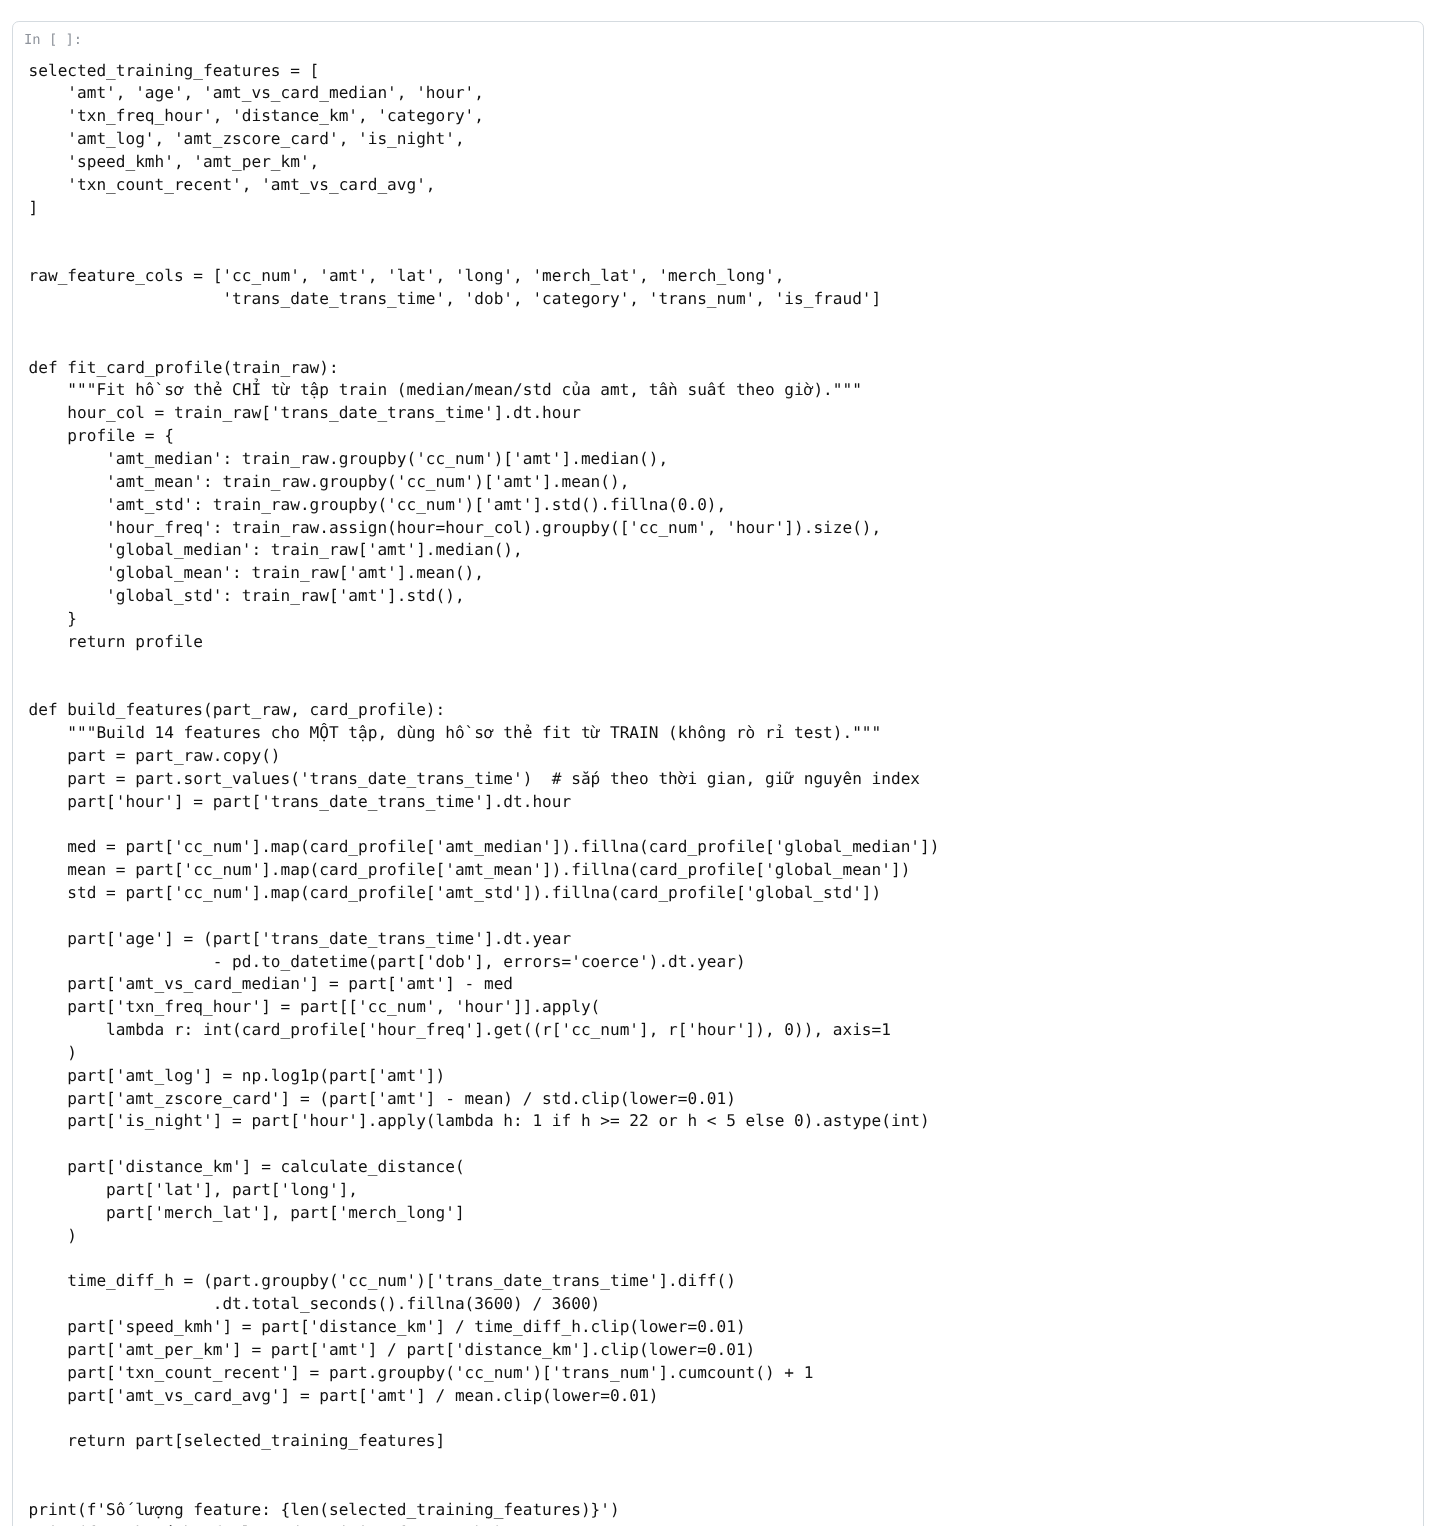
\includegraphics[width=\linewidth,height=0.9\textheight,keepaspectratio]{figures/code_features_1.png}
    \caption{Đoạn chương trình tạo các đặc trưng hành vi}
    \label{fig:code_features}
\end{figure}

Tóm lại, bài toán phân loại giao dịch thẻ tín dụng được phát biểu như sau: đầu vào là một giao dịch được mô tả bằng 14 đặc trưng gồm các giá trị số như số tiền, tuổi, giờ giao dịch, tần suất giao dịch, khoảng cách và tốc độ di chuyển, cũng như loại hình dịch vụ; đầu ra là nhãn phân loại 0 (giao dịch hợp lệ) hoặc 1 (giao dịch gian lận). Mô hình học máy trả về xác suất gian lận của từng giao dịch, sau đó ngưỡng quyết định được sử dụng để chuyển xác suất đó thành nhãn cuối cùng.

\chapter{PHÂN TÍCH KHÁM PHÁ DỮ LIỆU}
Phân tích khám phá giúp hiểu rõ cấu trúc dữ liệu, nhận diện các đặc điểm của giao dịch gian lận và phát hiện giá trị bất thường trước khi xây dựng mô hình. Quá trình này sử dụng các thư viện \texttt{seaborn} và \texttt{matplotlib} để trực quan hóa kết quả.

\section{Phân bố dữ liệu}
Hình \ref{fig:distributions} mô tả phân bố của ba đặc trưng số chính: logarit số tiền giao dịch \texttt{amt\_log}, tần suất giao dịch \texttt{txn\_freq\_hour} và khoảng cách \texttt{distance\_km}. Cả ba biến đều phân bố lệch về bên trái: phần lớn giao dịch có số tiền nhỏ, mỗi thẻ chỉ giao dịch một vài lần trong một giờ và khoảng cách từ đơn vị chấp nhận thanh toán đến vị trí thường trú của thẻ thường không quá 150 km. Phần đuôi dài bên phải của phân bố chứa các giá trị bất thường, nơi tập trung nhiều giao dịch gian lận.

\begin{figure}[H]
    \centering
    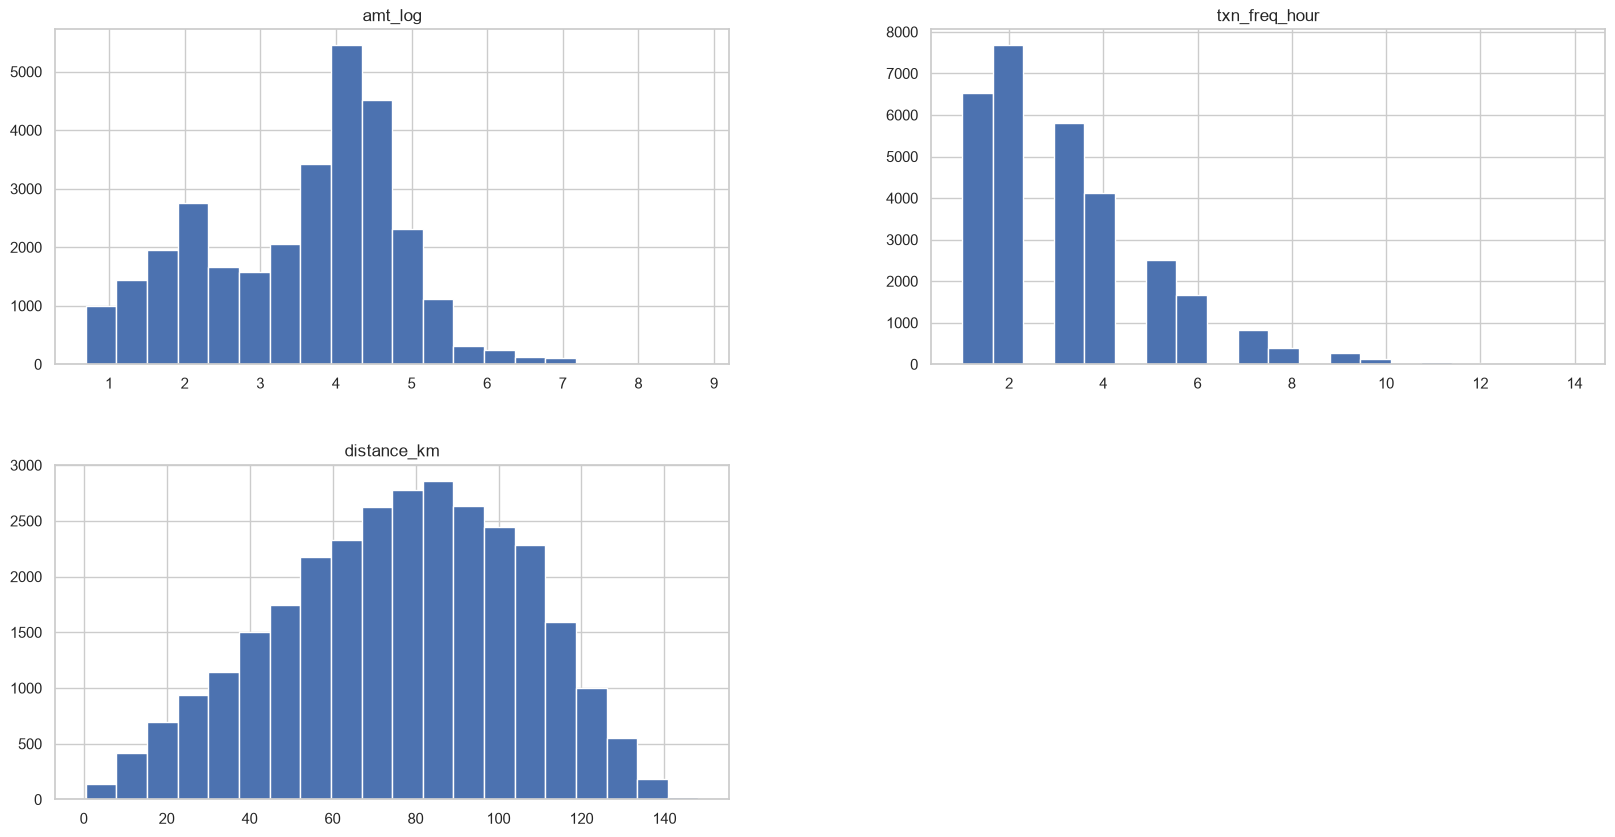
\includegraphics[width=1.0\linewidth]{figures/fig_distributions.png}
    \caption{Phân bố của các đặc trưng số trong bộ dữ liệu}
    \label{fig:distributions}
\end{figure}

\section{Gian lận theo loại hình dịch vụ}
Hình \ref{fig:fraud_category} thể hiện tỷ lệ gian lận của 10 loại hình dịch vụ có rủi ro cao nhất. Ba nhóm đầu là \texttt{shopping\_net}, \texttt{misc\_net} và \texttt{grocery\_pos} chiếm 82 trong tổng số 133 vụ gian lận, tương ứng 61{,}7\%. Loại \texttt{shopping\_net} có tỷ lệ gian lận cao nhất với 33 trong 2\,302 giao dịch, tương ứng 1{,}43\%, trong khi nhóm an toàn nhất \texttt{personal\_care} chỉ có 4 trong 2\,220 giao dịch, tương ứng 0{,}18\%. Kết quả kiểm định Chi-square cho giá trị $p = 1{,}28 \times 10^{-23}$, khẳng định loại hình dịch vụ có liên quan có ý nghĩa thống kê với gian lận, do đó \texttt{category} được giữ lại làm đặc trưng cho mô hình.

\begin{figure}[H]
    \centering
    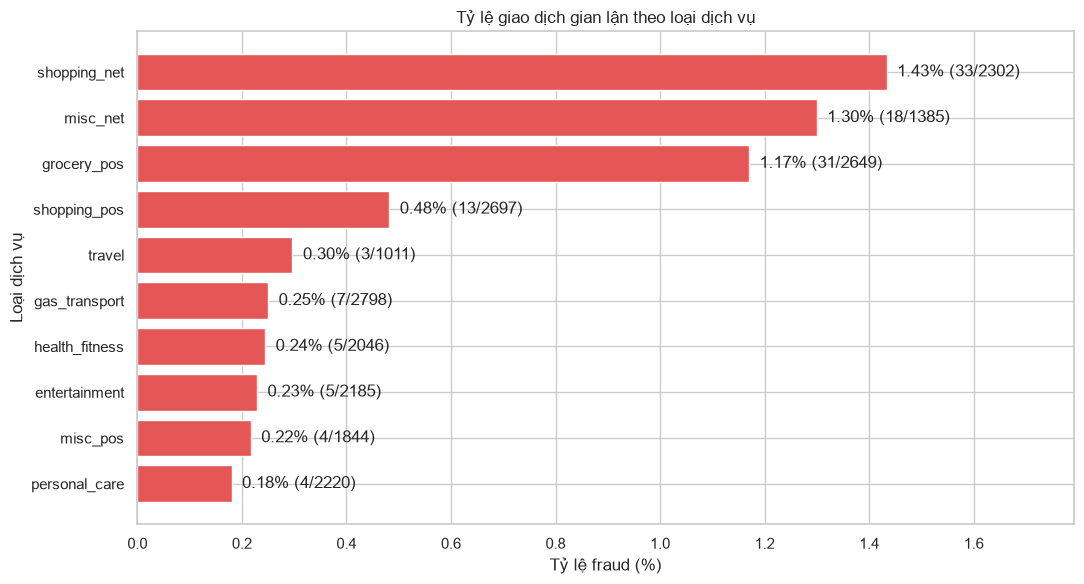
\includegraphics[width=0.9\linewidth]{figures/fig_fraud_category.png}
    \caption{Tỷ lệ giao dịch gian lận theo loại hình dịch vụ}
    \label{fig:fraud_category}
\end{figure}

\section{Giá trị bất thường}
Hình \ref{fig:outlier} dùng biểu đồ hộp để khảo sát giá trị bất thường của các đặc trưng số, và Bảng \ref{tab:outlier} thống kê chi tiết theo quy tắc $1{,}5 \times \text{IQR}$.

\begin{figure}[H]
    \centering
    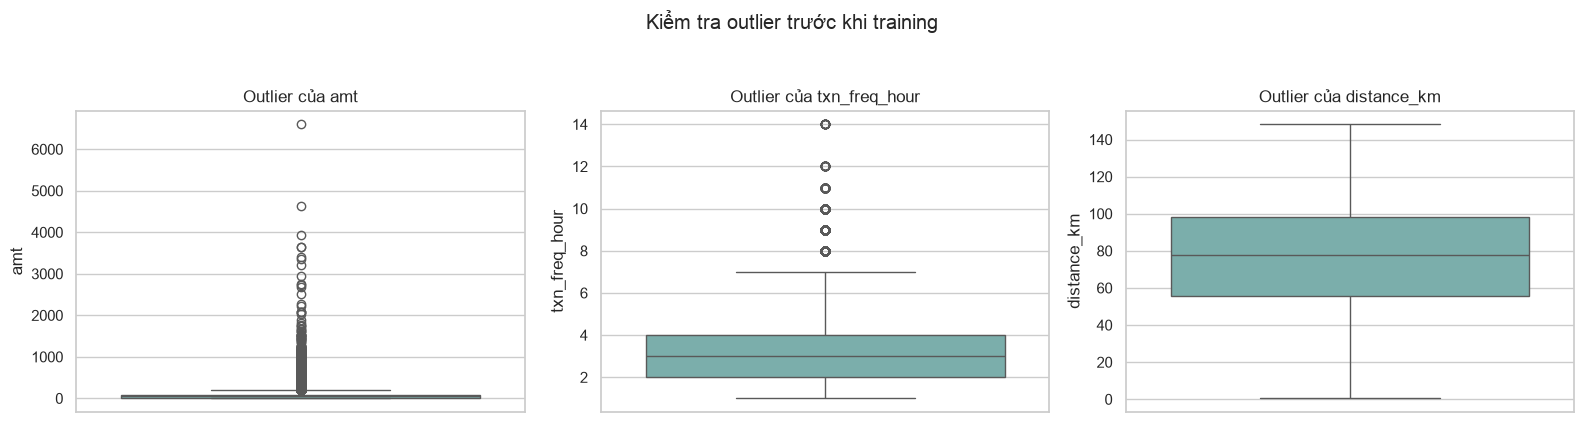
\includegraphics[width=1.0\linewidth]{figures/fig_outliers.png}
    \caption{Biểu đồ hộp kiểm tra giá trị bất thường}
    \label{fig:outlier}
\end{figure}

\begin{table}[H]
\centering
\fontsize{11}{13.6}\selectfont
\renewcommand{\arraystretch}{1.2}
\setlength{\tabcolsep}{6pt}
\begin{tabularx}{\textwidth}{|p{3.4cm}|p{2.5cm}|p{2.5cm}|X|}
\hline
\textbf{Đặc trưng} & \textbf{Ngưỡng trên} & \textbf{Số giá trị bất thường (tỷ lệ)} & \textbf{Gian lận trong vùng bất thường} \\
\hline
amt & 192{,}16 & 1\,521 (5{,}06\%) & 104 (78{,}2\%) \\
\hline
txn\_freq\_hour & 7{,}00 & 887 (2{,}95\%) & 5 \\
\hline
distance\_km & 162{,}10 & 0 (0\%) & 0 \\
\hline
\end{tabularx}
\caption{Thống kê giá trị bất thường theo quy tắc IQR}
\label{tab:outlier}
\end{table}

Đáng chú ý, 78{,}2\% số giao dịch gian lận nằm trong vùng giá trị bất thường của cột \texttt{amt}. Vì vậy, đồ án không xóa bỏ các giá trị bất thường ngay ở bước này mà chỉ giới hạn chúng theo quy tắc IQR sau khi chia tập huấn luyện và tập kiểm tra, nhằm tránh làm mất đi chính những giao dịch gian lận.



\section{Quan hệ giữa các đặc trưng}

\begin{figure}[H]
	\centering
	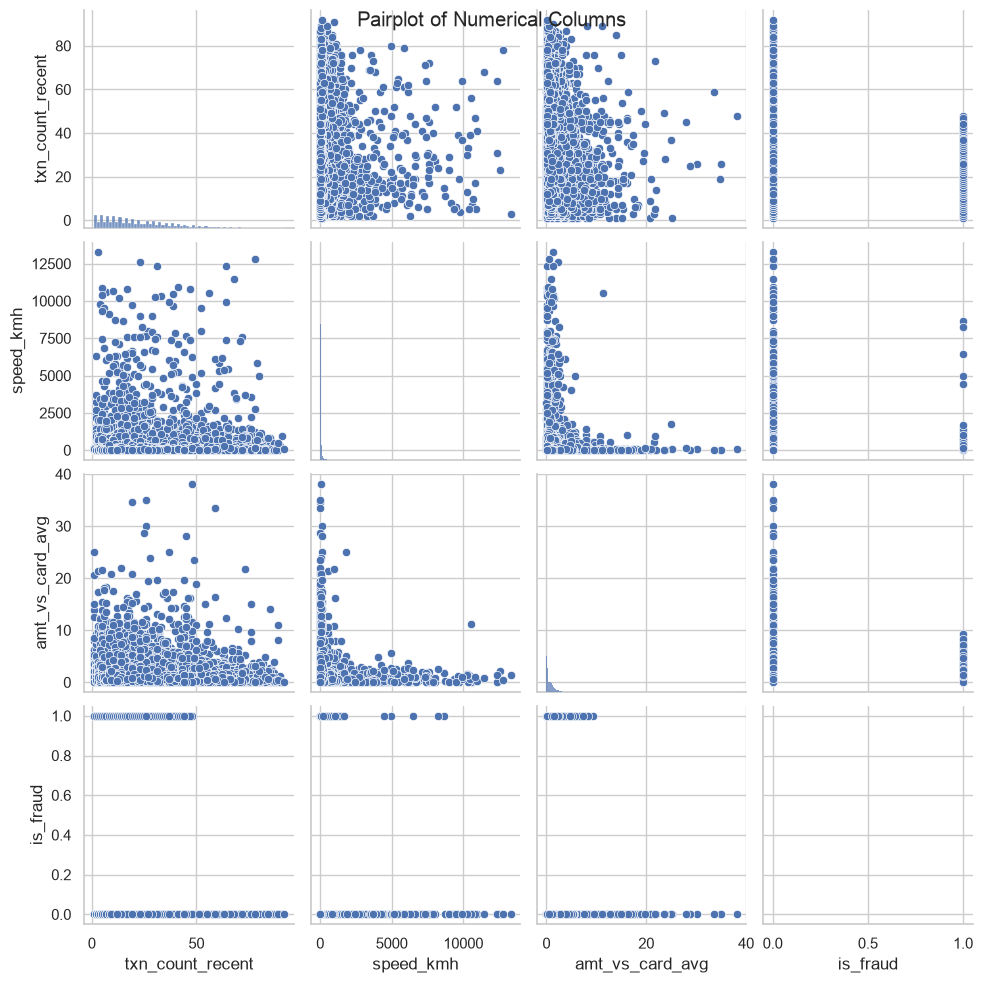
\includegraphics[width=0.9\linewidth]{figures/fig_scatter_features.png}
	\caption{Quan hệ cặp giữa các đặc trưng hành vi theo nhãn gian lận}
	\label{fig:scatter_features}
\end{figure}

Hình \ref{fig:scatter_features} trình bày quan hệ cặp giữa ba đặc trưng hành vi gồm số lần giao dịch gần đây \texttt{txn\_count\_recent}, tốc độ di chuyển \texttt{speed\_kmh} và tỷ lệ số tiền so với trung bình thẻ \texttt{amt\_vs\_card\_avg}, tô màu theo nhãn gian lận. Giao dịch gian lận có tốc độ di chuyển và tỷ lệ số tiền so với trung bình thẻ cao hơn rõ rệt: trung vị \texttt{speed\_kmh} là 59{,}4 km/h so với 21{,}2 km/h của giao dịch hợp lệ, trung vị \texttt{amt\_vs\_card\_avg} là 1{,}94 so với 0{,}67, cho thấy gian lận thường phát sinh ở nơi xa nơi ở quen thuộc và với số tiền vượt trung bình chi tiêu của thẻ. Ngược lại, \texttt{txn\_count\_recent} gần như không phân biệt hai lớp (trung vị 20 so với 19), nên chủ yếu đóng vai trò đặc trưng bổ trợ.



Qua các phân tích trên, 14 đặc trưng được chọn để đưa vào mô hình gồm: \texttt{amt}, \texttt{age}, \texttt{amt\_vs\_card\_median}, \texttt{hour}, \texttt{txn\_freq\_hour}, \texttt{distance\_km}, \texttt{category}, \texttt{amt\_log}, \texttt{amt\_zscore\_card}, \texttt{is\_night}, \texttt{speed\_kmh}, \texttt{amt\_per\_km}, \texttt{txn\_count\_recent} và \texttt{amt\_vs\_card\_avg}. Các cột định danh như \texttt{cc\_num} hay \texttt{trans\_num} không được dùng trực tiếp vì mô hình có thể học thuộc mã thay vì học quy luật tổng quát của gian lận.

\chapter{XÂY DỰNG CÁC MÔ HÌNH HỌC MÁY}
\section{Chuẩn bị dữ liệu cho mô hình}
\subsection{Tách đặc trưng và biến mục tiêu}
Từ bộ dữ liệu đã làm sạch, biến mục tiêu \texttt{is\_fraud} là nhãn gian lận được tách khỏi các đặc trưng đầu vào. Mười bốn đặc trưng được giữ lại gồm mười ba đặc trưng số \texttt{amt}, \texttt{age}, \texttt{amt\_vs\_card\_median}, \texttt{hour}, \texttt{txn\_freq\_hour}, \texttt{distance\_km}, \texttt{amt\_log}, \texttt{amt\_zscore\_card}, \texttt{is\_night}, \texttt{speed\_kmh}, \texttt{amt\_per\_km}, \texttt{txn\_count\_recent}, \texttt{amt\_vs\_card\_avg} và đặc trưng phân loại \texttt{category}. Đặc trưng phân loại \texttt{category} được mã hóa bằng \texttt{TargetEncoder}, tức mã hóa theo tương quan với biến mục tiêu, còn các đặc trưng số được chuẩn hóa về trung bình 0 và độ lệch chuẩn 1 bằng \texttt{StandardScaler}. Hai bước này được gói trong một \texttt{ColumnTransformer} \cite{pedregosa2011scikit} để đồng bộ giữa tập huấn luyện và tập kiểm tra.

\subsection{Chia tập dữ liệu}
Bộ dữ liệu 30\,058 giao dịch được chia theo tỷ lệ 80–20 bằng hàm \texttt{train\_test\_split} với \texttt{stratify = y} và \texttt{random\_state = 42}, cho tập huấn luyện 24\,046 mẫu, trong đó có 106 giao dịch gian lận, và tập kiểm tra 6\,012 mẫu, trong đó có 27 giao dịch gian lận. Tập huấn luyện được chia tiếp thành hai phần: phần Fit gồm 19\,236 mẫu, chiếm 80\%, dùng để huấn luyện và tinh chỉnh mô hình; phần Validation gồm 4\,810 mẫu, chiếm 20\%, dùng riêng để chọn ngưỡng quyết định. Tập kiểm tra chỉ được dùng đúng một lần để đánh giá cuối cùng.

Để tránh rò rỉ dữ liệu, mọi quy tắc học từ dữ liệu đều được tính riêng trên tập huấn luyện rồi mới áp dụng sang tập kiểm tra: giới hạn xử lý giá trị bất thường được suy ra từ tập huấn luyện, \texttt{StandardScaler} và \texttt{TargetEncoder} chỉ được học trên tập huấn luyện. Các giá trị bất thường của đặc trưng số được giới hạn theo quy tắc IQR tính trên tập huấn luyện thay vì bị xóa, vì giá trị bất thường có thể chính là giao dịch gian lận.

\section{Các chỉ số đánh giá mô hình}
Do tính chất mất cân bằng nghiêm trọng của dữ liệu, mô hình được đánh giá bằng các chỉ số Precision, Recall, F1-Score, F2-Score, ROC-AUC và PR-AUC:
\begin{align*}
\text{Precision} &= \frac{TP}{TP + FP}, \qquad
\text{Recall} = \frac{TP}{TP + FN}, \\
F1 &= \frac{2 \cdot \text{Precision} \cdot \text{Recall}}{\text{Precision} + \text{Recall}}, \qquad
F_\beta = (1 + \beta^2)\frac{\text{Precision} \cdot \text{Recall}}{\beta^2 \cdot \text{Precision} + \text{Recall}},
\end{align*}
trong đó $TP$, $FP$, $FN$ lần lượt là số giao dịch gian lận được phát hiện đúng, số giao dịch hợp lệ bị báo nhầm và số giao dịch gian lận bị bỏ sót. Ngoài ra, đồ án còn dùng ROC-AUC và PR-AUC; ROC-AUC đo khả năng phân biệt hai lớp theo xác suất, còn PR-AUC là diện tích dưới đường Precision--Recall và phù hợp hơn với dữ liệu mất cân bằng \cite{davis2006pr}.

Bởi vì bỏ sót giao dịch gian lận thường gây thiệt hại lớn hơn nhiều so với kiểm tra nhầm một giao dịch hợp lệ, chỉ số F2-Score với $\beta = 2$ được ưu tiên làm tiêu chí chính: chỉ số này đặt trọng số Recall gấp đôi Precision, khuyến khích mô hình phát hiện được nhiều gian lận hơn.

\section{Xử lý dữ liệu mất cân bằng}
Dữ liệu của đề tài có tỷ lệ mất cân bằng trên tập Fit là $\frac{19\,151}{85} \approx 225{:}1$ (kết quả tính từ dữ liệu của đồ án). Vì vậy, đồ án áp dụng bốn chiến lược xử lý dữ liệu mất cân bằng — một vấn đề phổ biến trong mô hình dự đoán trên dữ liệu mất cân bằng \cite{branco2016survey} — tương ứng với năm cấu hình mô hình, được trình bày trong Bảng \ref{tab:imbalance}.

\begin{table}[H]
\centering
\fontsize{11}{13.6}\selectfont
\renewcommand{\arraystretch}{1.2}
\setlength{\tabcolsep}{6pt}
\begin{tabularx}{\textwidth}{|p{3.4cm}|p{2.8cm}|X|}
\hline
\textbf{Chiến lược} & \textbf{Mô hình} & \textbf{Cách thiết lập} \\
\hline
Trọng số lớp & Random Forest & \texttt{class\_weight = "balanced"} hoặc trọng số thủ công $\{0{:}1,\ 1{:}k\}$ với $k \in \{20, 40, 60, 100, 150, 225\}$ \\
\hline
Trọng số lớp thiểu số & XGBoost, LightGBM & \texttt{scale\_pos\_weight} đặt quanh tỷ lệ mất cân bằng, gồm các mức 0{,}10; 0{,}25; 0{,}50; 0{,}75 và 1{,}0 lần tỷ lệ 225 \\
\hline
SMOTE nhẹ \cite{chawla2002smote} & XGBoost & Sinh thêm mẫu tổng hợp cho lớp gian lận với tỷ lệ thiểu số/đa số chỉ từ 2\% đến 5\%, thay vì cân bằng hoàn toàn \\
\hline
Trọng số tự động cân bằng & CatBoost & \texttt{auto\_class\_weights = "Balanced"}, trọng số nghịch đảo với tần suất của từng lớp \\
\hline
\end{tabularx}
\caption{Bốn chiến lược xử lý dữ liệu mất cân bằng}
\label{tab:imbalance}
\end{table}

Chiến lược SMOTE được đặt trong một \texttt{Pipeline} nhằm bảo đảm việc sinh dữ liệu tổng hợp chỉ diễn ra bên trong từng fold cross-validation, không làm rò rỉ thông tin vào tập xác thực.

\section{Lựa chọn ngưỡng quyết định}
Mô hình học máy trả về xác suất gian lận cho mỗi giao dịch. Thay vì dùng ngầm định ngưỡng 0{,}5, đồ án chọn ngưỡng tối ưu riêng cho từng mô hình trên tập Validation theo tiêu chí F2-Score cao nhất, đồng thời yêu cầu Precision tối thiểu 0{,}6 trên tập Validation để tránh cảnh báo tràn lan. Ràng buộc này được kiểm tra khi duyệt các ngưỡng ứng viên, nên ngưỡng cuối cùng chỉ được chọn trong vùng mà độ chính xác đã đủ cao; nếu một mô hình không đạt được ngưỡng này thì vẫn lấy ngưỡng có F2-Score cao nhất trong số các ngưỡng ứng viên. Cách tiếp cận này giúp ngưỡng được chọn độc lập với tập kiểm tra, và việc chỉ đánh giá một lần duy nhất trên tập kiểm tra giữ cho kết quả cuối cùng không bị lạc quan.

\section{Mô hình Random Forest}
Random Forest \cite{breiman2001randomforest} xây dựng nhiều cây quyết định trên các mẫu bootstrap khác nhau và lấy biểu quyết từ các cây, giúp giảm phương sai và ít bị ảnh hưởng bởi nhiễu. Không gian siêu tham số được khảo sát được trình bày trong Bảng \ref{tab:rf_params}. Điều chỉnh trọng số lớp kết hợp với giới hạn độ sâu giúp các cây tập trung hơn vào lớp thiểu số mà không quá khớp nhiễu.

\begin{table}[H]
\centering
\fontsize{11}{13.6}\selectfont
\renewcommand{\arraystretch}{1.2}
\setlength{\tabcolsep}{6pt}
\begin{tabularx}{\textwidth}{|p{4.8cm}|X|}
\hline
\textbf{Tham số} & \textbf{Giá trị khảo sát} \\
\hline
\texttt{n\_estimators} & số cây, từ 400 đến 1\,500 \\
\hline
\texttt{max\_depth} & None, 10, 15, 20, 25, 30, 40, 50 \\
\hline
\texttt{min\_samples\_split}, \texttt{min\_samples\_leaf} & ràng buộc kích thước nút và lá \\
\hline
\texttt{max\_features} & "sqrt", "log2", 0{,}3, 0{,}5, 0{,}7, 1{,}0 \\
\hline
\texttt{criterion} & "gini", "entropy", "log\_loss" \\
\hline
\texttt{class\_weight} & "balanced", "balanced\_subsample", $\{0{:}1,\ 1{:}k\}$ với $k = 20, 40, 60, 100, 150, 225$ \\
\hline
\end{tabularx}
\caption{Không gian siêu tham số của Random Forest}
\label{tab:rf_params}
\end{table}

\section{Mô hình XGBoost}
XGBoost \cite{chen2016xgboost} là thuật toán gradient boosting xây dựng các cây tuần tự, cây sau được huấn luyện để khắc phục sai lệch của các cây trước, kèm cơ chế chính quy hóa gồm \texttt{gamma}, \texttt{reg\_alpha} và \texttt{reg\_lambda} để chống quá khớp. Không gian siêu tham số được khảo sát được trình bày trong Bảng \ref{tab:xgb_params}.

\begin{table}[H]
\centering
\fontsize{11}{13.6}\selectfont
\renewcommand{\arraystretch}{1.2}
\setlength{\tabcolsep}{6pt}
\begin{tabularx}{\textwidth}{|p{4.8cm}|X|}
\hline
\textbf{Tham số} & \textbf{Giá trị khảo sát} \\
\hline
\texttt{n\_estimators} & số cây, từ 300 đến 1\,500 \\
\hline
\texttt{max\_depth} & độ sâu tối đa, từ 2 đến 10 \\
\hline
\texttt{learning\_rate} & tốc độ học, từ 0{,}005 đến 0{,}15 \\
\hline
\texttt{subsample}, \texttt{colsample\_bytree} & tỷ lệ mẫu và đặc trưng dùng cho mỗi cây, từ 0{,}55 đến 1{,}00 \\
\hline
\texttt{min\_child\_weight} & trọng số tối thiểu của nút con, từ 1 đến 20 \\
\hline
\texttt{gamma} & ngưỡng suy giảm lỗi tối thiểu để tách nút, từ 0 đến 2 \\
\hline
\texttt{reg\_alpha}, \texttt{reg\_lambda} & hệ số chính quy hóa L1 và L2 \\
\hline
\texttt{scale\_pos\_weight} & trọng số lớp gian lận: 1; $\sqrt{225}$; 0{,}10; 0{,}25; 0{,}50; 0{,}75; 1{,}00 lần tỷ lệ mất cân bằng \\
\hline
\end{tabularx}
\caption{Không gian siêu tham số của XGBoost}
\label{tab:xgb_params}
\end{table}

\section{Mô hình LightGBM}
LightGBM \cite{ke2017lightgbm} là thuật toán gradient boosting dùng bộ phân tách dựa trên hướng (histogram-based), cho phép huấn luyện nhanh trên dữ liệu lớn và tự xử lý mất cân bằng lớp bằng tham số \texttt{scale\_pos\_weight} \cite{lightgbmparameters}. Không gian siêu tham số được khảo sát được trình bày trong Bảng \ref{tab:lgbm_params}.

\begin{table}[H]
\centering
\fontsize{11}{13.6}\selectfont
\renewcommand{\arraystretch}{1.2}
\setlength{\tabcolsep}{6pt}
\begin{tabularx}{\textwidth}{|p{4.8cm}|X|}
\hline
\textbf{Tham số} & \textbf{Giá trị khảo sát} \\
\hline
\texttt{n\_estimators} & số cây, từ 300 đến 1\,500 \\
\hline
\texttt{max\_depth} & độ sâu tối đa, từ 3 đến 12 \\
\hline
\texttt{num\_leaves} & số lá trên mỗi cây, từ 15 đến 64 \\
\hline
\texttt{learning\_rate} & tốc độ học, từ 0{,}005 đến 0{,}15 \\
\hline
\texttt{min\_child\_samples} & số mẫu tối thiểu của một nút lá, từ 5 đến 50 \\
\hline
\texttt{subsample}, \texttt{colsample\_bytree} & tỷ lệ mẫu và đặc trưng dùng cho mỗi cây, từ 0{,}55 đến 1{,}00 \\
\hline
\texttt{reg\_alpha}, \texttt{reg\_lambda} & hệ số chính quy hóa L1 và L2 \\
\hline
\texttt{scale\_pos\_weight} & trọng số lớp gian lận: 1; $\sqrt{225}$; 0{,}25; 0{,}50; 0{,}75; 1{,}00 lần tỷ lệ mất cân bằng \\
\hline
\end{tabularx}
\caption{Không gian siêu tham số của LightGBM}
\label{tab:lgbm_params}
\end{table}

\subsection{Cấu hình tối ưu của LightGBM}
Sau khi \texttt{RandomizedSearchCV} với 60 lần thử trên cross-validation 5-fold, LightGBM đạt điểm PR-AUC cross-validation cao nhất là 0{,}8525, vượt trội so với bốn cấu hình còn lại. Bộ siêu tham số tương ứng được trình bày ở Bảng \ref{tab:lgbm_best}. Cấu hình này dùng \texttt{scale\_pos\_weight} bằng 15{,}01, tức nhẹ hơn đáng kể so với tỷ lệ mất cân bằng đầy đủ là 225{,}31, cho thấy việc tăng trọng số lớp thiểu số vừa đủ giúp mô hình tập trung vào lớp gian lận mà không làm méo quá mức phân phối xác suất. Số cây 1\,483 đi kèm tốc độ học thấp 0{,}0314 là một cấu hình hội tụ chậm, vốn là lựa chọn phổ biến cho bài toán dữ liệu nhỏ và mất cân bằng.

\begin{table}[H]
\centering
\fontsize{10.5}{12.6}\selectfont
\renewcommand{\arraystretch}{1.05}
\setlength{\tabcolsep}{9pt}
\begin{tabular}{|>{\raggedright\arraybackslash}p{4.1cm}|>{\centering\arraybackslash}p{2.9cm}|}
\hline
\textbf{Tham số} & \textbf{Giá trị tối ưu} \\
\hline
\texttt{n\_estimators} & 1\,483 \\
\hline
\texttt{learning\_rate} & 0{,}0314 \\
\hline
\texttt{num\_leaves} & 21 \\
\hline
\texttt{max\_depth} & 6 \\
\hline
\texttt{min\_child\_samples} & 17 \\
\hline
\texttt{subsample} & 0{,}8310 \\
\hline
\texttt{colsample\_bytree} & 0{,}8220 \\
\hline
\texttt{reg\_alpha} & 0{,}00281 \\
\hline
\texttt{reg\_lambda} & 0{,}13136 \\
\hline
\texttt{scale\_pos\_weight} & 15{,}01 \\
\hline
\end{tabular}
\caption{Bộ siêu tham số tối ưu của LightGBM theo \texttt{RandomizedSearchCV}}
\label{tab:lgbm_best}
\end{table}

Với cấu hình này, chênh lệch giữa điểm PR-AUC cross-validation trên tập Fit là 0{,}8525 và điểm PR-AUC trên tập kiểm tra là 0{,}8197 ở mức 0{,}0328, cho thấy mức độ quá khớp ở mức chấp nhận được và không cần dựng thêm biến thể giảm quá khớp. Kết quả chi tiết của cấu hình này trên tập kiểm tra được trình bày ở Bảng \ref{tab:exp3} của chương đánh giá.

\section{Mô hình CatBoost}
CatBoost \cite{prokhorenkova2018catboost} là thuật toán gradient boosting xử lý đặc trưng phân loại bên trong cây, dùng trọng số tự động cân bằng lớp \texttt{auto\_class\_weights = "Balanced"} để đối phó với dữ liệu mất cân bằng mà không cần điều chỉnh thủ công. Không gian siêu tham số được khảo sát được trình bày trong Bảng \ref{tab:cat_params}.

\begin{table}[H]
\centering
\fontsize{11}{13.6}\selectfont
\renewcommand{\arraystretch}{1.2}
\setlength{\tabcolsep}{6pt}
\begin{tabularx}{\textwidth}{|p{4.8cm}|X|}
\hline
\textbf{Tham số} & \textbf{Giá trị khảo sát} \\
\hline
\texttt{iterations} & số vòng huấn luyện, từ 300 đến 1\,200 \\
\hline
\texttt{depth} & độ sâu tối đa, từ 4 đến 10 \\
\hline
\texttt{learning\_rate} & tốc độ học, từ 0{,}005 đến 0{,}15 \\
\hline
\texttt{l2\_leaf\_reg} & hệ số chính quy hóa L2, từ 0{,}1 đến 10 \\
\hline
\texttt{bagging\_temperature}, \texttt{random\_strength} & mức ngẫu nhiên khi lấy mẫu và khi chọn ranh giới phân hoạch \\
\hline
\texttt{border\_count} & số ngưỡng phân hoạch liên tục, từ 32 đến 255 \\
\hline
\texttt{min\_data\_in\_leaf} & số mẫu tối thiểu của một nút lá, từ 1 đến 20 \\
\hline
\end{tabularx}
\caption{Không gian siêu tham số của CatBoost}
\label{tab:cat_params}
\end{table}

\section{Kết hợp mô hình bằng Stacking}
Sau khi tinh chỉnh, ba cấu hình có điểm F2-Score trên tập Validation cao nhất được chọn làm mô hình cơ sở (base learners), gồm XGBoost--trọng số, LightGBM và CatBoost. Các mô hình cơ sở được kết hợp bằng \texttt{StackingClassifier} \cite{wolpert1992stacked}: mỗi mô hình cơ sở sinh xác suất gian lận trên các fold cross-validation 3 lớp, xác suất này được đưa vào bộ tổng hợp (meta-learner) là một hồi quy Logistic có trọng số lớp cân bằng để học cách kết hợp các mô hình sao cho F2-Score cao nhất. Bước kết hợp này giúp mô hình tận dụng điểm mạnh từng mô hình và giảm phụ thuộc vào một cấu hình duy nhất.

\section{Quá trình tinh chỉnh siêu tham số}
Năm cấu hình Random Forest, XGBoost--trọng số, XGBoost--SMOTE nhẹ, LightGBM và CatBoost đều được tinh chỉnh bằng \texttt{RandomizedSearchCV} \cite{sklearnrandomizedsearch} với cross-validation 5-fold trên các đặc trưng đã mã hóa bằng TargetEncoder. Hàm tính điểm là \texttt{average\_precision}, tương ứng với Average Precision (AP), một thước đo dựa trên đường Precision--Recall nhằm thích ứng với dữ liệu mất cân bằng \cite{sklearnaverageprecision}. Số lần thử ngẫu nhiên là 80 cho Random Forest, 80 cho mỗi cấu hình XGBoost, 60 cho LightGBM và 40 cho CatBoost, với \texttt{random\_state = 42} để kết quả tái lập được. Kết quả cross-validation của từng cấu hình được trình bày trong Bảng \ref{tab:cv_results}. LightGBM với \texttt{scale\_pos\_weight} vượt trội rõ rệt so với bốn cấu hình còn lại, dẫn đầu về PR-AUC với 0{,}8525. Quy trình tinh chỉnh trên được cố định cho toàn bộ sáu thử nghiệm ở chương đánh giá; giữa các thử nghiệm chỉ có tập đặc trưng đầu vào thay đổi, nhờ đó mọi so sánh đều không bị ảnh hưởng bởi khác biệt về ngân sách tìm kiếm siêu tham số.

\begin{table}[H]
\centering
\fontsize{11}{13.6}\selectfont
\renewcommand{\arraystretch}{1.2}
\setlength{\tabcolsep}{6pt}
\begin{tabularx}{\textwidth}{|>{\raggedright\arraybackslash}p{5.2cm}|>{\centering\arraybackslash}p{2.2cm}|>{\centering\arraybackslash}X|}
\hline
\textbf{Cấu hình} & \textbf{Số lần thử} & \textbf{Điểm PR-AUC tốt nhất (5-fold)} \\
\hline
Random Forest & 80 & 0{,}7555 \\
\hline
XGBoost (Scale Pos Weight) & 80 & 0{,}7973 \\
\hline
XGBoost (Light SMOTE) & 80 & 0{,}7642 \\
\hline
LightGBM (Scale Pos Weight) & 60 & 0{,}8525 \\
\hline
CatBoost (Auto class weights) & 40 & 0{,}7883 \\
\hline
\end{tabularx}
\caption{Số lần thử và điểm PR-AUC cross-validation tốt nhất của từng cấu hình}
\label{tab:cv_results}
\end{table}

\chapter{ĐÁNH GIÁ VÀ THẢO LUẬN KẾT QUẢ}
\section{Phạm vi sáu thử nghiệm}
Để đánh giá ảnh hưởng của cách biểu diễn đặc trưng và của việc loại bỏ đặc trưng nhiễu, đề tài thiết kế sáu thử nghiệm. Tất cả thử nghiệm dùng chung một cách chia tập dữ liệu (tập Fit 19\,236 mẫu -- Validation 4\,810 mẫu -- tập kiểm tra 6\,012 mẫu), cùng một bộ thuật toán và cùng một quy trình tinh chỉnh siêu tham số; chỉ có tập đặc trưng đầu vào là thay đổi. Ngưỡng quyết định của mỗi cấu hình được chọn trên tập Validation theo F2-Score với Precision tối thiểu 0{.}6, rồi mới đánh giá một lần duy nhất trên tập kiểm tra gồm 6\,012 giao dịch, trong đó có 27 giao dịch gian lận và 5\,985 giao dịch hợp lệ.

Bên cạnh các chỉ số đã trình bày ở phần trước, mỗi bảng kết quả dưới đây báo cáo thêm hai tỷ lệ lỗi phản ánh trực tiếp rủi ro của hệ thống. Tỷ lệ bỏ sót gian lận, viết tắt FNR, là tỷ lệ giao dịch gian lận thật không bị phát hiện; tỷ lệ báo nhầm giao dịch hợp lệ, viết tắt FPR, là tỷ lệ giao dịch hợp lệ bị cảnh báo nhầm là gian lận. Sáu thử nghiệm được tóm tắt trong Bảng \ref{tab:exp_setup}.

\begin{table}[H]
\centering
\fontsize{11}{13.6}\selectfont
\renewcommand{\arraystretch}{1.2}
\setlength{\tabcolsep}{5pt}
\begin{tabularx}{\textwidth}{|>{\centering\arraybackslash}p{1.5cm}|>{\raggedright\arraybackslash}p{4.6cm}|>{\centering\arraybackslash}p{1.7cm}|X|}
\hline
\textbf{Thử nghiệm} & \textbf{Cách biểu diễn đặc trưng} & \textbf{Số đặc trưng} & \textbf{Mô hình được huấn luyện} \\
\hline
TN1 & Sáu đặc trưng gốc, chưa tạo đặc trưng mới & 6 & Random Forest, XGBoost \\
\hline
TN2 & \texttt{OneHotEncoder} cho đặc trưng phân loại & 26 & CatBoost, LightGBM, XGBoost, Random Forest \\
\hline
TN3 & \texttt{TargetEncoder} cho đặc trưng phân loại & 14 & LightGBM, Stacking, Random Forest, XGBoost, CatBoost \\
\hline
TN4 & thử nghiệm3 trừ \texttt{is\_night}, \texttt{amt\_vs\_card\_median}, \texttt{distance\_km}, \texttt{amt} & 10 & Stacking, LightGBM, XGBoost, Random Forest, CatBoost \\
\hline
TN5 & thử nghiệm3 trừ \texttt{is\_night}, \texttt{amt\_vs\_card\_median}, \texttt{distance\_km} & 11 & LightGBM, XGBoost, Random Forest, CatBoost \\
\hline
TN6 & thử nghiệm3 trừ \texttt{amt}, \texttt{amt\_vs\_card\_median}, \texttt{distance\_km} & 11 & XGBoost, LightGBM, CatBoost, Random Forest \\
\hline
\end{tabularx}
\caption{Sáu thử nghiệm đánh giá ảnh hưởng của cách mã hóa và của việc loại bỏ đặc trưng}
\label{tab:exp_setup}
\end{table}

Ba thử nghiệm đầu (TN1--TN3) giữ nguyên tập đặc trưng và chỉ thay đổi cách biểu diễn, nhằm tách ảnh hưởng của phương pháp mã hóa. Ba thử nghiệm sau (TN4--TN6) lấy thử nghiệm3 làm chuẩn và loại bỏ dần các đặc trưng mà phân tích khám phá cho thấy chứa nhiễu, nhằm kiểm tra liệu việc giảm số chiều có làm mô hình tốt hơn hay không.

\section{Kết quả từng thử nghiệm}
\subsection{Thử nghiệm 1: sáu đặc trưng gốc}
Khi chỉ dùng sáu đặc trưng gốc mà không tạo thêm đặc trưng, hiệu quả của các mô hình giảm mạnh. Random Forest đạt PR-AUC 0{.}5016 và F1-Score 0{.}5319, trong khi XGBoost thấp hơn với PR-AUC 0{.}4141. Nguyên nhân là các đặc trưng thô chưa diễn đạt được mối quan hệ phi tuyến giữa số tiền giao dịch và hành vi của chủ thẻ --- ví dụ số tiền so với mức trung bình của chính thẻ đó --- là những tín hiệu mạnh nhất trong dữ liệu. Đây là cơ sở để đề tài bổ sung nhóm đặc trưng kỹ thuật ở phần trước.

\begin{table}[H]
\centering
\fontsize{11}{13.6}\selectfont
\renewcommand{\arraystretch}{1.2}
\setlength{\tabcolsep}{4pt}
\begin{tabularx}{\textwidth}{|>{\raggedright\arraybackslash}X|>{\centering\arraybackslash}p{1.35cm}|>{\centering\arraybackslash}p{1.58cm}|>{\centering\arraybackslash}p{1.22cm}|>{\centering\arraybackslash}p{1.15cm}|>{\centering\arraybackslash}p{1.15cm}|>{\centering\arraybackslash}p{1.25cm}|>{\centering\arraybackslash}p{1.25cm}|>{\centering\arraybackslash}p{1.15cm}|>{\centering\arraybackslash}p{1.2cm}|}
\hline
\textbf{Mô hình} & \textbf{Ngưỡng} & \textbf{Precision} & \textbf{Recall} & \textbf{F1} & \textbf{F2} & \textbf{ROC-AUC} & \textbf{PR-AUC} & \textbf{FNR} & \textbf{FPR} \\
\hline
Random Forest & 0{.}1464 & 0{.}5682 & 0{.}5000 & 0{.}5319 & 0{.}5123 & 0{.}9261 & 0{.}5016 & 0{.}5000 & 0{.}0043 \\
\hline
XGBoost & 0{.}0422 & 0{.}3506 & 0{.}5400 & 0{.}4252 & 0{.}4874 & 0{.}9567 & 0{.}4141 & 0{.}4600 & 0{.}0112 \\
\hline
\end{tabularx}
\caption{Kết quả thử nghiệm1 trên tập kiểm tra với sáu đặc trưng gốc}
\label{tab:exp1}
\end{table}

\subsection{Thử nghiệm 2: mã hóa One-Hot}
Mã hóa \texttt{OneHotEncoder} làm số đặc trưng tăng lên 26 và hiệu quả tăng vượt bậc so với thử nghiệm1. Tuy nhiên đây chưa phải cấu hình tốt nhất: LightGBM đạt PR-AUC 0{.}8092 với F2-Score 0{.}7554, trong khi CatBoost đạt F2-Score cao hơn là 0{.}7801 nhờ Recall 0{.}8148, đổi lại Precision chỉ 0{.}6667. Điểm đáng chú ý là thời gian tinh chỉnh siêu tham số của LightGBM trong cấu hình này lên tới 1\,143{.}26 giây, cao hơn gấp đôi so với các thử nghiệm sau, do không gian mã hóa rời rạc làm tìm kiếm chậm hơn.

\begin{table}[H]
\centering
\fontsize{11}{13.6}\selectfont
\renewcommand{\arraystretch}{1.2}
\setlength{\tabcolsep}{4pt}
\begin{tabularx}{\textwidth}{|>{\raggedright\arraybackslash}X|>{\centering\arraybackslash}p{1.35cm}|>{\centering\arraybackslash}p{1.58cm}|>{\centering\arraybackslash}p{1.22cm}|>{\centering\arraybackslash}p{1.15cm}|>{\centering\arraybackslash}p{1.15cm}|>{\centering\arraybackslash}p{1.25cm}|>{\centering\arraybackslash}p{1.25cm}|>{\centering\arraybackslash}p{1.15cm}|>{\centering\arraybackslash}p{1.2cm}|}
\hline
\textbf{Mô hình} & \textbf{Ngưỡng} & \textbf{Precision} & \textbf{Recall} & \textbf{F1} & \textbf{F2} & \textbf{ROC-AUC} & \textbf{PR-AUC} & \textbf{FNR} & \textbf{FPR} \\
\hline
CatBoost & 0{.}6186 & 0{.}6667 & 0{.}8148 & 0{.}7333 & 0{.}7801 & 0{.}9673 & 0{.}7821 & 0{.}1852 & 0{.}0018 \\
\hline
LightGBM & 0{.}0553 & 0{.}6774 & 0{.}7778 & 0{.}7241 & 0{.}7554 & 0{.}9756 & 0{.}8092 & 0{.}2222 & 0{.}0017 \\
\hline
XGBoost & 0{.}2858 & 0{.}7143 & 0{.}7407 & 0{.}7273 & 0{.}7353 & 0{.}9721 & 0{.}7693 & 0{.}2593 & 0{.}0013 \\
\hline
Random Forest & 0{.}2100 & 0{.}7600 & 0{.}7037 & 0{.}7308 & 0{.}7143 & 0{.}9727 & 0{.}7765 & 0{.}2963 & 0{.}0010 \\
\hline
\end{tabularx}
\caption{Kết quả thử nghiệm2 trên tập kiểm tra với mã hóa \texttt{OneHotEncoder} (26 đặc trưng)}
\label{tab:exp2}
\end{table}

\subsection{Thử nghiệm 3: mã hóa Target Encoder}
Thay \texttt{OneHotEncoder} bằng \texttt{TargetEncoder} thu gọn tập đặc trưng còn 14 chiều và cho kết quả cân bằng nhất trong sáu thử nghiệm. LightGBM với \texttt{scale\_pos\_weight} đạt PR-AUC 0{.}8197, F1-Score 0{.}8163 và F2-Score 0{.}7692 --- đều là giá trị cao nhất --- với Precision 0{.}9091, Recall 0{.}7407, FPR chỉ 0{.}0003 và thời gian dự đoán 0{.}0361 giây. Stacking chỉ đứng thứ hai về PR-AUC (0{.}7820): mô hình này bắt được 21 trong 27 vụ gian lận, nhiều hơn LightGBM đúng 1 vụ, nhưng đổi lại phải báo nhầm 9 giao dịch hợp lệ so với chỉ 2 giao dịch, nên xét cả hai loại rủi ro thì Stacking không tốt bằng LightGBM.

\begin{table}[H]
\centering
\fontsize{11}{13.6}\selectfont
\renewcommand{\arraystretch}{1.2}
\setlength{\tabcolsep}{4pt}
\begin{tabularx}{\textwidth}{|>{\raggedright\arraybackslash}X|>{\centering\arraybackslash}p{1.35cm}|>{\centering\arraybackslash}p{1.58cm}|>{\centering\arraybackslash}p{1.22cm}|>{\centering\arraybackslash}p{1.15cm}|>{\centering\arraybackslash}p{1.15cm}|>{\centering\arraybackslash}p{1.25cm}|>{\centering\arraybackslash}p{1.25cm}|>{\centering\arraybackslash}p{1.15cm}|>{\centering\arraybackslash}p{1.2cm}|}
\hline
\textbf{Mô hình} & \textbf{Ngưỡng} & \textbf{Precision} & \textbf{Recall} & \textbf{F1} & \textbf{F2} & \textbf{ROC-AUC} & \textbf{PR-AUC} & \textbf{FNR} & \textbf{FPR} \\
\hline
LightGBM & 0{.}0634 & 0{.}9091 & 0{.}7407 & 0{.}8163 & 0{.}7692 & 0{.}9828 & 0{.}8197 & 0{.}2593 & 0{.}0003 \\
\hline
Stacking & 0{.}9827 & 0{.}7000 & 0{.}7778 & 0{.}7368 & 0{.}7609 & 0{.}9598 & 0{.}7820 & 0{.}2222 & 0{.}0015 \\
\hline
Random Forest & 0{.}2498 & 0{.}6897 & 0{.}7407 & 0{.}7143 & 0{.}7299 & 0{.}9516 & 0{.}7475 & 0{.}2593 & 0{.}0015 \\
\hline
XGBoost & 0{.}2545 & 0{.}5882 & 0{.}7407 & 0{.}6557 & 0{.}7042 & 0{.}9758 & 0{.}7398 & 0{.}2593 & 0{.}0023 \\
\hline
CatBoost & 0{.}8407 & 0{.}3922 & 0{.}7407 & 0{.}5128 & 0{.}6289 & 0{.}9711 & 0{.}6895 & 0{.}2593 & 0{.}0052 \\
\hline
\end{tabularx}
\caption{Kết quả thử nghiệm3 trên tập kiểm tra với mã hóa \texttt{TargetEncoder} (14 đặc trưng)}
\label{tab:exp3}
\end{table}

\subsection{Thử nghiệm 4: loại bỏ bốn đặc trưng}
Thử nghiệm 4 loại bỏ bốn đặc trưng gồm \texttt{is\_night}, \texttt{amt\_vs\_card\_median}, \texttt{distance\_km} và \texttt{amt}, còn 10 đặc trưng. LightGBM đạt PR-AUC 0{.}8231, cao nhất trong toàn bộ sáu thử nghiệm, và F1-Score 0{.}8000 gần bằng thử nghiệm 3. Tuy nhiên F2-Score giảm xuống 0{.}7634, Precision giảm còn 0{.}8696, FPR tăng gấp rưỡi lên 0{.}0005, thời gian dự đoán tăng lên 0{.}1048 giây và thời gian tinh chỉnh tăng vọt lên 2\,235{.}59 giây. Việc loại bỏ \texttt{amt} làm mô hình mất tín hiệu số tiền tuyệt đối, vốn là đặc trưng có ảnh hưởng lớn nhất theo phân tích mức độ ảnh hưởng của các đặc trưng trình bày tại Hình \ref{fig:perm_imp}.

\begin{table}[H]
\centering
\fontsize{11}{13.6}\selectfont
\renewcommand{\arraystretch}{1.2}
\setlength{\tabcolsep}{4pt}
\begin{tabularx}{\textwidth}{|>{\raggedright\arraybackslash}X|>{\centering\arraybackslash}p{1.35cm}|>{\centering\arraybackslash}p{1.58cm}|>{\centering\arraybackslash}p{1.22cm}|>{\centering\arraybackslash}p{1.15cm}|>{\centering\arraybackslash}p{1.15cm}|>{\centering\arraybackslash}p{1.25cm}|>{\centering\arraybackslash}p{1.25cm}|>{\centering\arraybackslash}p{1.15cm}|>{\centering\arraybackslash}p{1.2cm}|}
\hline
\textbf{Mô hình} & \textbf{Ngưỡng} & \textbf{Precision} & \textbf{Recall} & \textbf{F1} & \textbf{F2} & \textbf{ROC-AUC} & \textbf{PR-AUC} & \textbf{FNR} & \textbf{FPR} \\
\hline
Stacking & 0{.}9910 & 0{.}7500 & 0{.}7778 & 0{.}7636 & 0{.}7721 & 0{.}9705 & 0{.}7819 & 0{.}2222 & 0{.}0012 \\
\hline
LightGBM & 0{.}0480 & 0{.}8696 & 0{.}7407 & 0{.}8000 & 0{.}7634 & 0{.}9826 & 0{.}8231 & 0{.}2593 & 0{.}0005 \\
\hline
XGBoost & 0{.}5840 & 0{.}9048 & 0{.}7037 & 0{.}7917 & 0{.}7364 & 0{.}9808 & 0{.}7338 & 0{.}2963 & 0{.}0003 \\
\hline
Random Forest & 0{.}1387 & 0{.}5882 & 0{.}7407 & 0{.}6557 & 0{.}7042 & 0{.}9673 & 0{.}7416 & 0{.}2593 & 0{.}0023 \\
\hline
CatBoost & 0{.}8407 & 0{.}3922 & 0{.}7407 & 0{.}5128 & 0{.}6289 & 0{.}9711 & 0{.}6895 & 0{.}2593 & 0{.}0052 \\
\hline
\end{tabularx}
\caption{Kết quả thử nghiệm4 trên tập kiểm tra sau khi loại bỏ bốn đặc trưng (10 đặc trưng)}
\label{tab:exp4}
\end{table}

\subsection{Thử nghiệm 5: loại bỏ \texttt{is\_night}, \texttt{amt\_vs\_card\_median}, \texttt{distance\_km}}
Thử nghiệm 5 giữ lại \texttt{amt} nhưng loại bỏ \texttt{is\_night}, \texttt{amt\_vs\_card\_median} và \texttt{distance\_km}, còn 11 đặc trưng. LightGBM đạt PR-AUC 0{.}8205, gần bằng thử nghiệm 3, nhưng Recall giảm mạnh xuống 0{.}6667 nên F1-Score (0{.}7660) và F2-Score (0{.}7031) đều thấp hơn đáng kể, kéo theo FNR tăng lên 0{.}3333 tức bỏ sót 9 trong 27 giao dịch gian lận. Trong bốn thử nghiệm còn lại, XGBoost và CatBoost đều có PR-AUC dưới 0{.}76 và thấp hơn đáng kể so với LightGBM.

\begin{table}[H]
\centering
\fontsize{11}{13.6}\selectfont
\renewcommand{\arraystretch}{1.2}
\setlength{\tabcolsep}{4pt}
\begin{tabularx}{\textwidth}{|>{\raggedright\arraybackslash}X|>{\centering\arraybackslash}p{1.35cm}|>{\centering\arraybackslash}p{1.58cm}|>{\centering\arraybackslash}p{1.22cm}|>{\centering\arraybackslash}p{1.15cm}|>{\centering\arraybackslash}p{1.15cm}|>{\centering\arraybackslash}p{1.25cm}|>{\centering\arraybackslash}p{1.25cm}|>{\centering\arraybackslash}p{1.15cm}|>{\centering\arraybackslash}p{1.2cm}|}
\hline
\textbf{Mô hình} & \textbf{Ngưỡng} & \textbf{Precision} & \textbf{Recall} & \textbf{F1} & \textbf{F2} & \textbf{ROC-AUC} & \textbf{PR-AUC} & \textbf{FNR} & \textbf{FPR} \\
\hline
LightGBM & 0{.}1840 & 0{.}9000 & 0{.}6667 & 0{.}7660 & 0{.}7031 & 0{.}9845 & 0{.}8205 & 0{.}3333 & 0{.}0003 \\
\hline
XGBoost & 0{.}2234 & 0{.}4884 & 0{.}7778 & 0{.}6000 & 0{.}6954 & 0{.}9721 & 0{.}7584 & 0{.}2222 & 0{.}0037 \\
\hline
Random Forest & 0{.}1266 & 0{.}5405 & 0{.}7407 & 0{.}6250 & 0{.}6897 & 0{.}9478 & 0{.}7465 & 0{.}2593 & 0{.}0028 \\
\hline
CatBoost & 0{.}4779 & 0{.}6333 & 0{.}7037 & 0{.}6667 & 0{.}6884 & 0{.}9754 & 0{.}7816 & 0{.}2963 & 0{.}0018 \\
\hline
\end{tabularx}
\caption{Kết quả thử nghiệm5 trên tập kiểm tra sau khi loại bỏ ba đặc trưng (11 đặc trưng)}
\label{tab:exp5}
\end{table}

\subsection{Thử nghiệm 6: loại bỏ \texttt{amt}, \texttt{amt\_vs\_card\_median}, \texttt{distance\_km}}
Thử nghiệm 6 cũng còn 11 đặc trưng nhưng giữ lại \texttt{is\_night} thay cho \texttt{amt}. LightGBM đạt PR-AUC 0{.}8068, thấp hơn thử nghiệm 3 và là cấu hình LightGBM yếu nhất trong năm thử nghiệm; F2-Score 0{.}7364 và FNR 0{.}2963 đều kém hơn. XGBoost trong thử nghiệm 6 đạt F1 và F2 bằng nhau là 0{.}7407 do ngưỡng 0{.}2600 đặt trùng vị trí phân loại, cho thấy hiệu quả của XGBoost phụ thuộc mạnh vào tập đặc trưng hơn LightGBM.

\begin{table}[H]
\centering
\fontsize{11}{13.6}\selectfont
\renewcommand{\arraystretch}{1.2}
\setlength{\tabcolsep}{4pt}
\begin{tabularx}{\textwidth}{|>{\raggedright\arraybackslash}X|>{\centering\arraybackslash}p{1.35cm}|>{\centering\arraybackslash}p{1.58cm}|>{\centering\arraybackslash}p{1.22cm}|>{\centering\arraybackslash}p{1.15cm}|>{\centering\arraybackslash}p{1.15cm}|>{\centering\arraybackslash}p{1.25cm}|>{\centering\arraybackslash}p{1.25cm}|>{\centering\arraybackslash}p{1.15cm}|>{\centering\arraybackslash}p{1.2cm}|}
\hline
\textbf{Mô hình} & \textbf{Ngưỡng} & \textbf{Precision} & \textbf{Recall} & \textbf{F1} & \textbf{F2} & \textbf{ROC-AUC} & \textbf{PR-AUC} & \textbf{FNR} & \textbf{FPR} \\
\hline
XGBoost & 0{.}2600 & 0{.}7407 & 0{.}7407 & 0{.}7407 & 0{.}7407 & 0{.}9628 & 0{.}7480 & 0{.}2593 & 0{.}0012 \\
\hline
LightGBM & 0{.}2666 & 0{.}9048 & 0{.}7037 & 0{.}7917 & 0{.}7364 & 0{.}9808 & 0{.}8068 & 0{.}2963 & 0{.}0003 \\
\hline
CatBoost & 0{.}9023 & 0{.}8571 & 0{.}6667 & 0{.}7500 & 0{.}6977 & 0{.}9754 & 0{.}7579 & 0{.}3333 & 0{.}0005 \\
\hline
Random Forest & 0{.}1321 & 0{.}5405 & 0{.}7407 & 0{.}6250 & 0{.}6897 & 0{.}9461 & 0{.}7297 & 0{.}2593 & 0{.}0028 \\
\hline
\end{tabularx}
\caption{Kết quả thử nghiệm6 trên tập kiểm tra sau khi loại bỏ ba đặc trưng (11 đặc trưng)}
\label{tab:exp6}
\end{table}

\section{Giải thích ảnh hưởng của các đặc trưng}
Để giải thích vì sao các thử nghiệm loại bỏ đặc trưng lại cho kết quả như vậy, đề tài đo mức độ ảnh hưởng của từng đặc trưng theo phương pháp hoán đổi ngẫu nhiên, thực hiện bằng hàm \texttt{permutation\_importance} của thư viện \texttt{scikit-learn} \cite{scikitlearnpermutation}. Cụ thể, mỗi đặc trưng được hoán đổi ngẫu nhiên 10 lần và đo mức giảm PR-AUC, lấy trung bình trên 10 lần lặp. Phương pháp này đáng tin cậy hơn chỉ số độ quan trọng sẵn có của mô hình cây vì đo trực tiếp ảnh hưởng thực tế lên chất lượng dự đoán, thay vì chỉ đo mức độ chia nút. Hình \ref{fig:perm_imp} trình bày kết quả cho mô hình LightGBM tại cấu hình tốt nhất của thử nghiệm 3.

\begin{figure}[H]
    \centering
    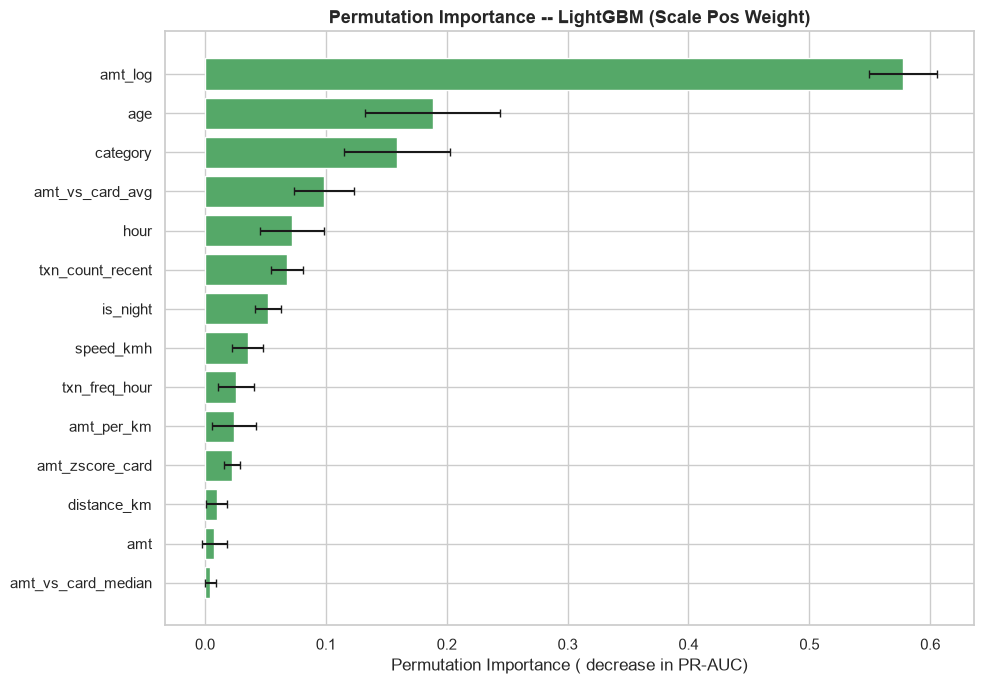
\includegraphics[width=0.9\linewidth]{figures/fig_permutation_importance_lightgbm.png}
    \caption{Mức độ ảnh hưởng của 14 đặc trưng theo phương pháp hoán đổi ngẫu nhiên, đo trên tập Validation}
    \label{fig:perm_imp}
\end{figure}

Hình \ref{fig:perm_imp} cho thấy \texttt{amt\_log} áp đảo với mức ảnh hưởng 0{.}5778, lớn hơn tổng của bốn đặc trưng đứng kế tiếp và gấp 3{.}1 lần \texttt{age} (0{.}1883); tiếp theo là \texttt{category} (0{.}1591), \texttt{amt\_vs\_card\_avg} (0{.}0982) và \texttt{hour} (0{.}0716). Ở cuối bảng là \texttt{amt\_vs\_card\_median} (0{.}0043), \texttt{amt} (0{.}0077) và \texttt{distance\_km} (0{.}0095), tức gần như không đóng góp. Kết quả này giải thích trực tiếp cho toàn bộ sáu thử nghiệm:

\begin{itemize}
    \item Vì \texttt{amt\_log} là biến dẫn xuất từ \texttt{amt}, nên khi thử nghiệm 4 loại bỏ \texttt{amt} thì đặc trưng mạnh nhất cũng biến mất, giải thích việc F2-Score và Precision của thử nghiệm 4 đều thấp hơn thử nghiệm 3.
    \item Hai đặc trưng \texttt{distance\_km} và \texttt{amt\_vs\_card\_median} có ảnh hưởng gần bằng không, nên việc loại bỏ chúng ở thử nghiệm 5 và thử nghiệm 6 không mang lại lợi ích rõ ràng --- đồng thời cho thấy chúng chỉ gây nhiễu nhẹ chứ không phải nguồn nhiễu nghiêm trọng.
    \item \texttt{is\_night} có ảnh hưởng 0{.}0521, thuộc nhóm giữa và lớn hơn rõ rệt ba đặc trưng gần như vô dụng kể trên, nên thử nghiệm 5 loại bỏ nó đã làm Recall giảm từ 0{.}7407 xuống 0{.}6667.
    \item Ba đặc trưng \texttt{is\_night}, \texttt{amt\_vs\_card\_median} và \texttt{distance\_km} mà ba thử nghiệm cuối loại bỏ có tổng ảnh hưởng chỉ khoảng 0{.}066, thấp hơn nhiều so với \texttt{amt\_log}; đây là lý do kết luận rằng việc loại bỏ đặc trưng không làm mô hình tốt hơn là có cơ sở định lượng chứ không chỉ là quan sát thực nghiệm.
\end{itemize}

\section{Tổng hợp và so sánh sáu thử nghiệm}
Bảng \ref{tab:exp_summary} và Hình \ref{fig:exp_compare} tổng hợp cấu hình tốt nhất của từng thử nghiệm. Ba kết luận nổi bật:

\begin{itemize}
    \item Kỹ thuật tạo đặc trưng quan trọng hơn phương pháp mã hóa. So sánh thử nghiệm 1 với thử nghiệm 3 cho thấy PR-AUC tăng từ 0{.}5016 lên 0{.}8197, tức tăng 63\%, chỉ nhờ bổ sung nhóm đặc trưng kỹ thuật. Trong khi đó, thay \texttt{OneHotEncoder} bằng \texttt{TargetEncoder} (thử nghiệm 2 $\to$ thử nghiệm 3) chỉ cải thiện PR-AUC từ 0{.}8092 lên 0{.}8197 nhưng lại giảm số chiều từ 26 xuống 14, giảm thời gian tinh chỉnh từ 1\,143{.}26 giây xuống 231{.}85 giây và tăng Precision từ 0{.}6774 lên 0{.}9091.
    \item Loại bỏ đặc trưng không làm mô hình tốt hơn. Cả ba thử nghiệm thử nghiệm 4--thử nghiệm 6 đều có PR-AUC của LightGBM cao hơn thử nghiệm 3 một chút (0{.}8231; 0{.}8205; 0{.}8068) nhưng đều tệ hơn ở F1-Score hoặc F2-Score, đồng thời tốn thời gian dự đoán và tinh chỉnh nhiều hơn. Chênh lệch PR-AUC giữa thử nghiệm3 và thử nghiệm4 chỉ là 0{.}0034, nhỏ hơn nhiều so với sai số do chỉ có 27 giao dịch gian lận trong tập kiểm tra: đổi số dự đoán đúng của một điểm Recall là 1/27 $\approx$ 0{.}037. Vì vậy, việc loại bỏ đặc trưng không mang lại lợi ích có ý nghĩa, và tập 14 đặc trưng của thử nghiệm3 được giữ lại.
    \item LightGBM là thuật toán bền vững nhất. Trong năm thử nghiệm có LightGBM, mô hình này dẫn đầu về PR-AUC ở cả năm thử nghiệm, đồng thời luôn giữ FPR ở mức 0{.}0003--0{.}0017, thấp hơn hẳn CatBoost (tới 0{.}0052) và XGBoost (tới 0{.}0037). Ngược lại, hiệu quả của XGBoost, CatBoost và Random Forest biến động mạnh theo tập đặc trưng: CatBoost rơi từ PR-AUC 0{.}7821 ở thử nghiệm2 xuống 0{.}6895 ở thử nghiệm3 và thử nghiệm4; XGBoost giảm từ 0{.}7693 xuống 0{.}7398.
\end{itemize}

\begin{table}[H]
\centering
\fontsize{10}{12.5}\selectfont
\renewcommand{\arraystretch}{1.2}
\setlength{\tabcolsep}{4pt}
\begin{adjustbox}{max width=\textwidth}
\begin{tabular}{|>{\centering\arraybackslash}p{1.25cm}|>{\raggedright\arraybackslash}p{3.4cm}|>{\centering\arraybackslash}p{1.2cm}|>{\centering\arraybackslash}p{1.58cm}|>{\centering\arraybackslash}p{1.22cm}|>{\centering\arraybackslash}p{1.1cm}|>{\centering\arraybackslash}p{1.1cm}|>{\centering\arraybackslash}p{1.35cm}|>{\centering\arraybackslash}p{1.45cm}|}
\hline
\textbf{TN} & \textbf{Cấu hình tốt nhất} & \textbf{Số đặc trưng} & \textbf{Precision} & \textbf{Recall} & \textbf{F1} & \textbf{F2} & \textbf{PR-AUC} & \textbf{Thời gian (s)} \\
\hline
TN1 & Random Forest & 6 & 0{.}5682 & 0{.}5000 & 0{.}5319 & 0{.}5123 & 0{.}5016 & 1{.}8849 \\
\hline
TN2 & LightGBM & 26 & 0{.}6774 & 0{.}7778 & 0{.}7241 & 0{.}7554 & 0{.}8092 & 0{.}1349 \\
\hline
TN3 & LightGBM & 14 & 0{.}9091 & 0{.}7407 & 0{.}8163 & 0{.}7692 & 0{.}8197 & 0{.}0361 \\
\hline
TN4 & LightGBM & 10 & 0{.}8696 & 0{.}7407 & 0{.}8000 & 0{.}7634 & 0{.}8231 & 0{.}1048 \\
\hline
TN5 & LightGBM & 11 & 0{.}9000 & 0{.}6667 & 0{.}7660 & 0{.}7031 & 0{.}8205 & 0{.}0941 \\
\hline
TN6 & LightGBM & 11 & 0{.}9048 & 0{.}7037 & 0{.}7917 & 0{.}7364 & 0{.}8068 & 0{.}0499 \\
\hline
\end{tabular}
\end{adjustbox}
\caption{Cấu hình tốt nhất của từng thử nghiệm trên tập kiểm tra. Với thử nghiệm1, cột thời gian ghi thời gian huấn luyện cuối cùng thay vì thời gian dự đoán, do đó không so sánh trực tiếp với năm thử nghiệm còn lại.}
\label{tab:exp_summary}
\end{table}

\begin{figure}[H]
    \centering
    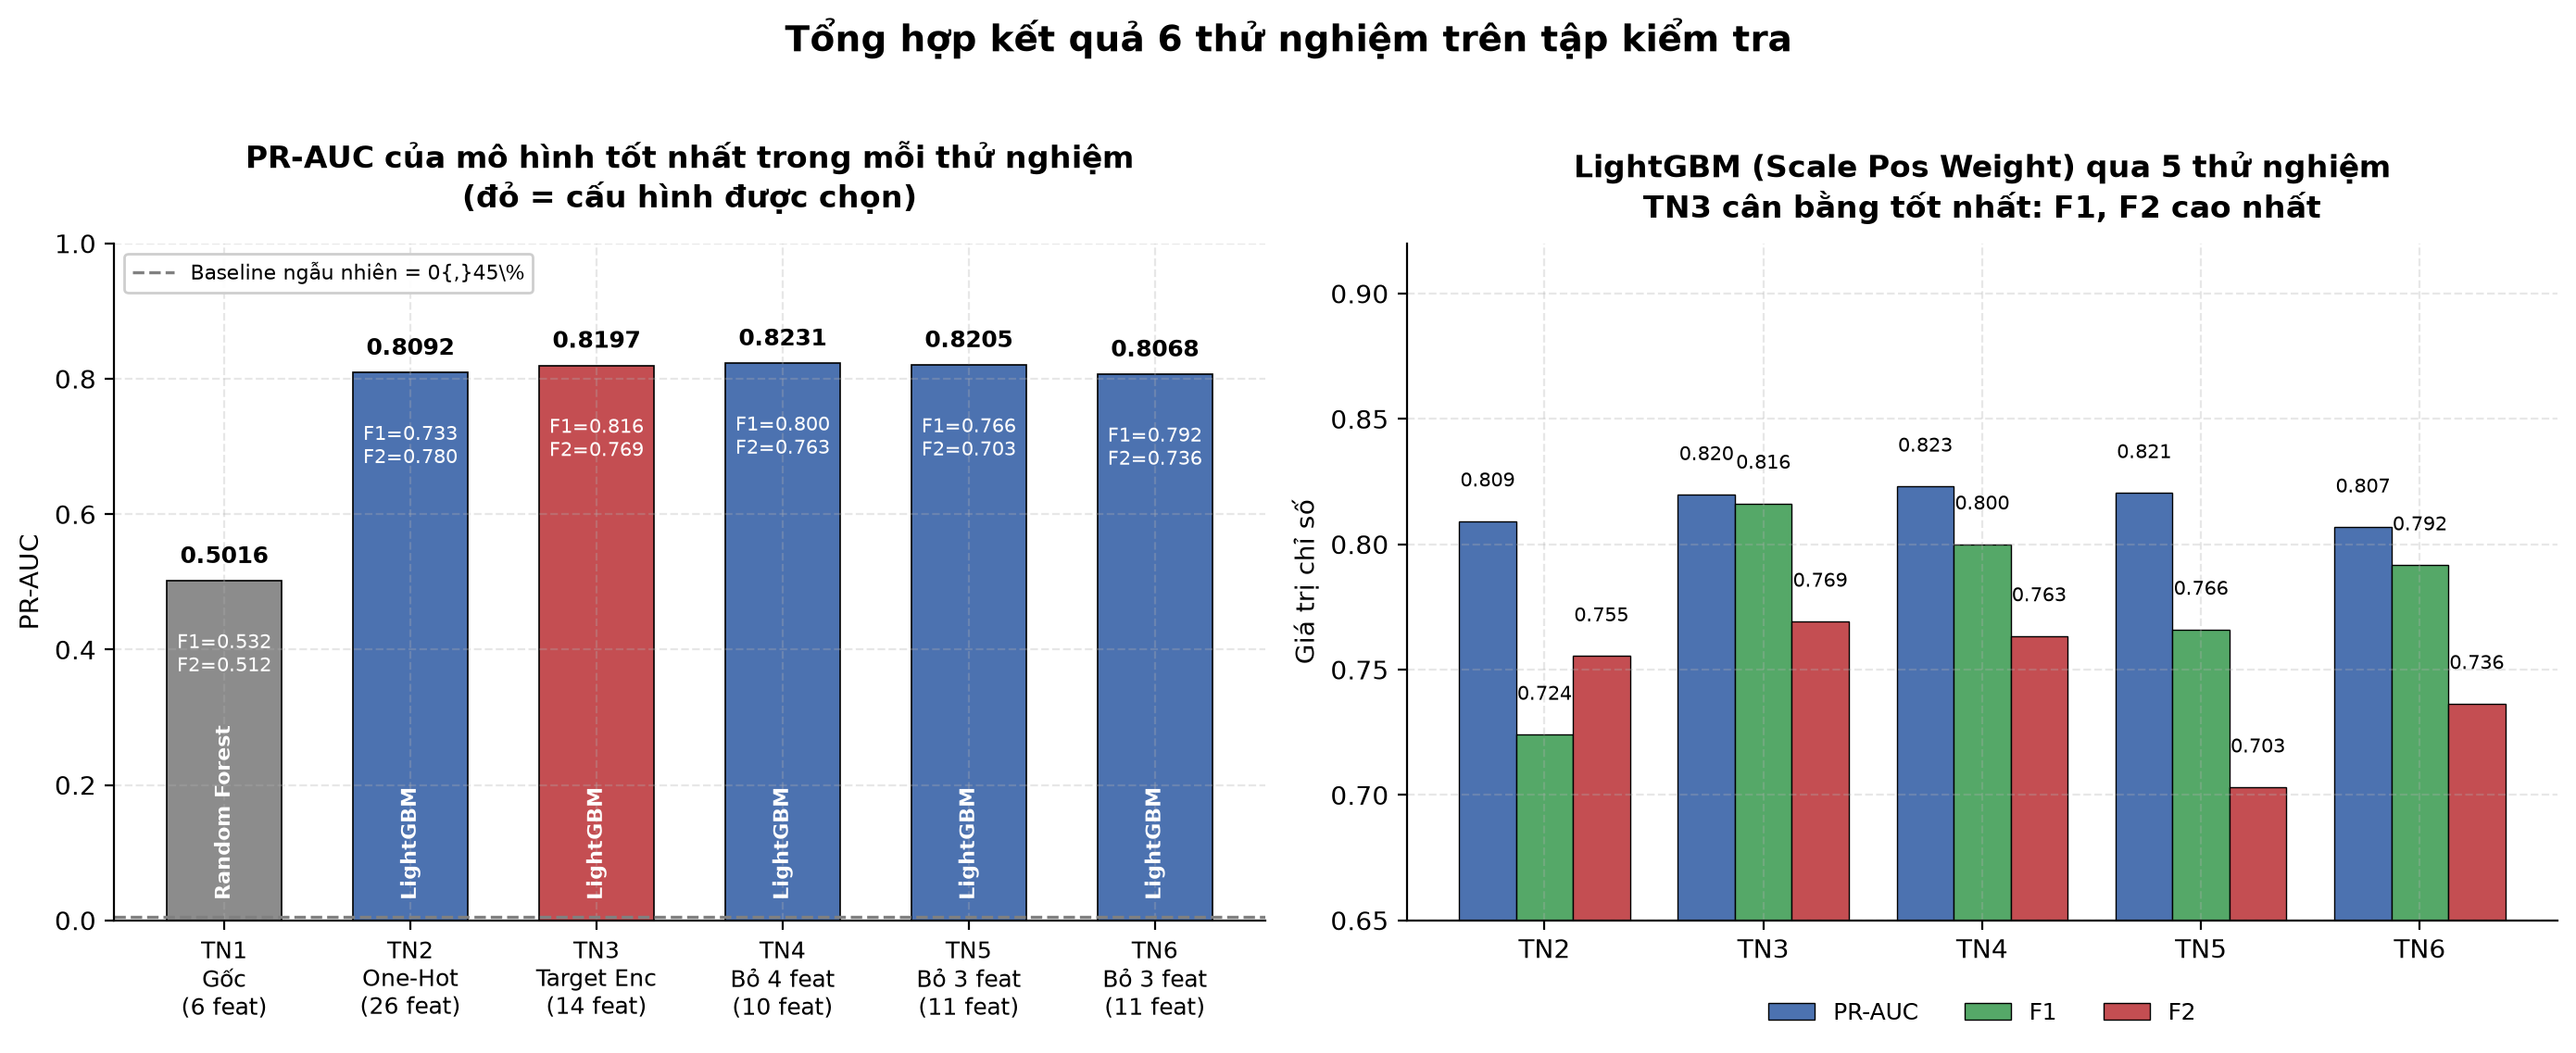
\includegraphics[width=\linewidth]{figures/fig_experiment_compare.png}
    \caption{So sánh PR-AUC của cấu hình tốt nhất trong sáu thử nghiệm (trái) và hiệu quả của LightGBM qua năm thử nghiệm (phải)}
    \label{fig:exp_compare}
\end{figure}

\section{Ma trận nhầm lẫn và đường Precision--Recall}
\begin{figure}[H]
    \centering
    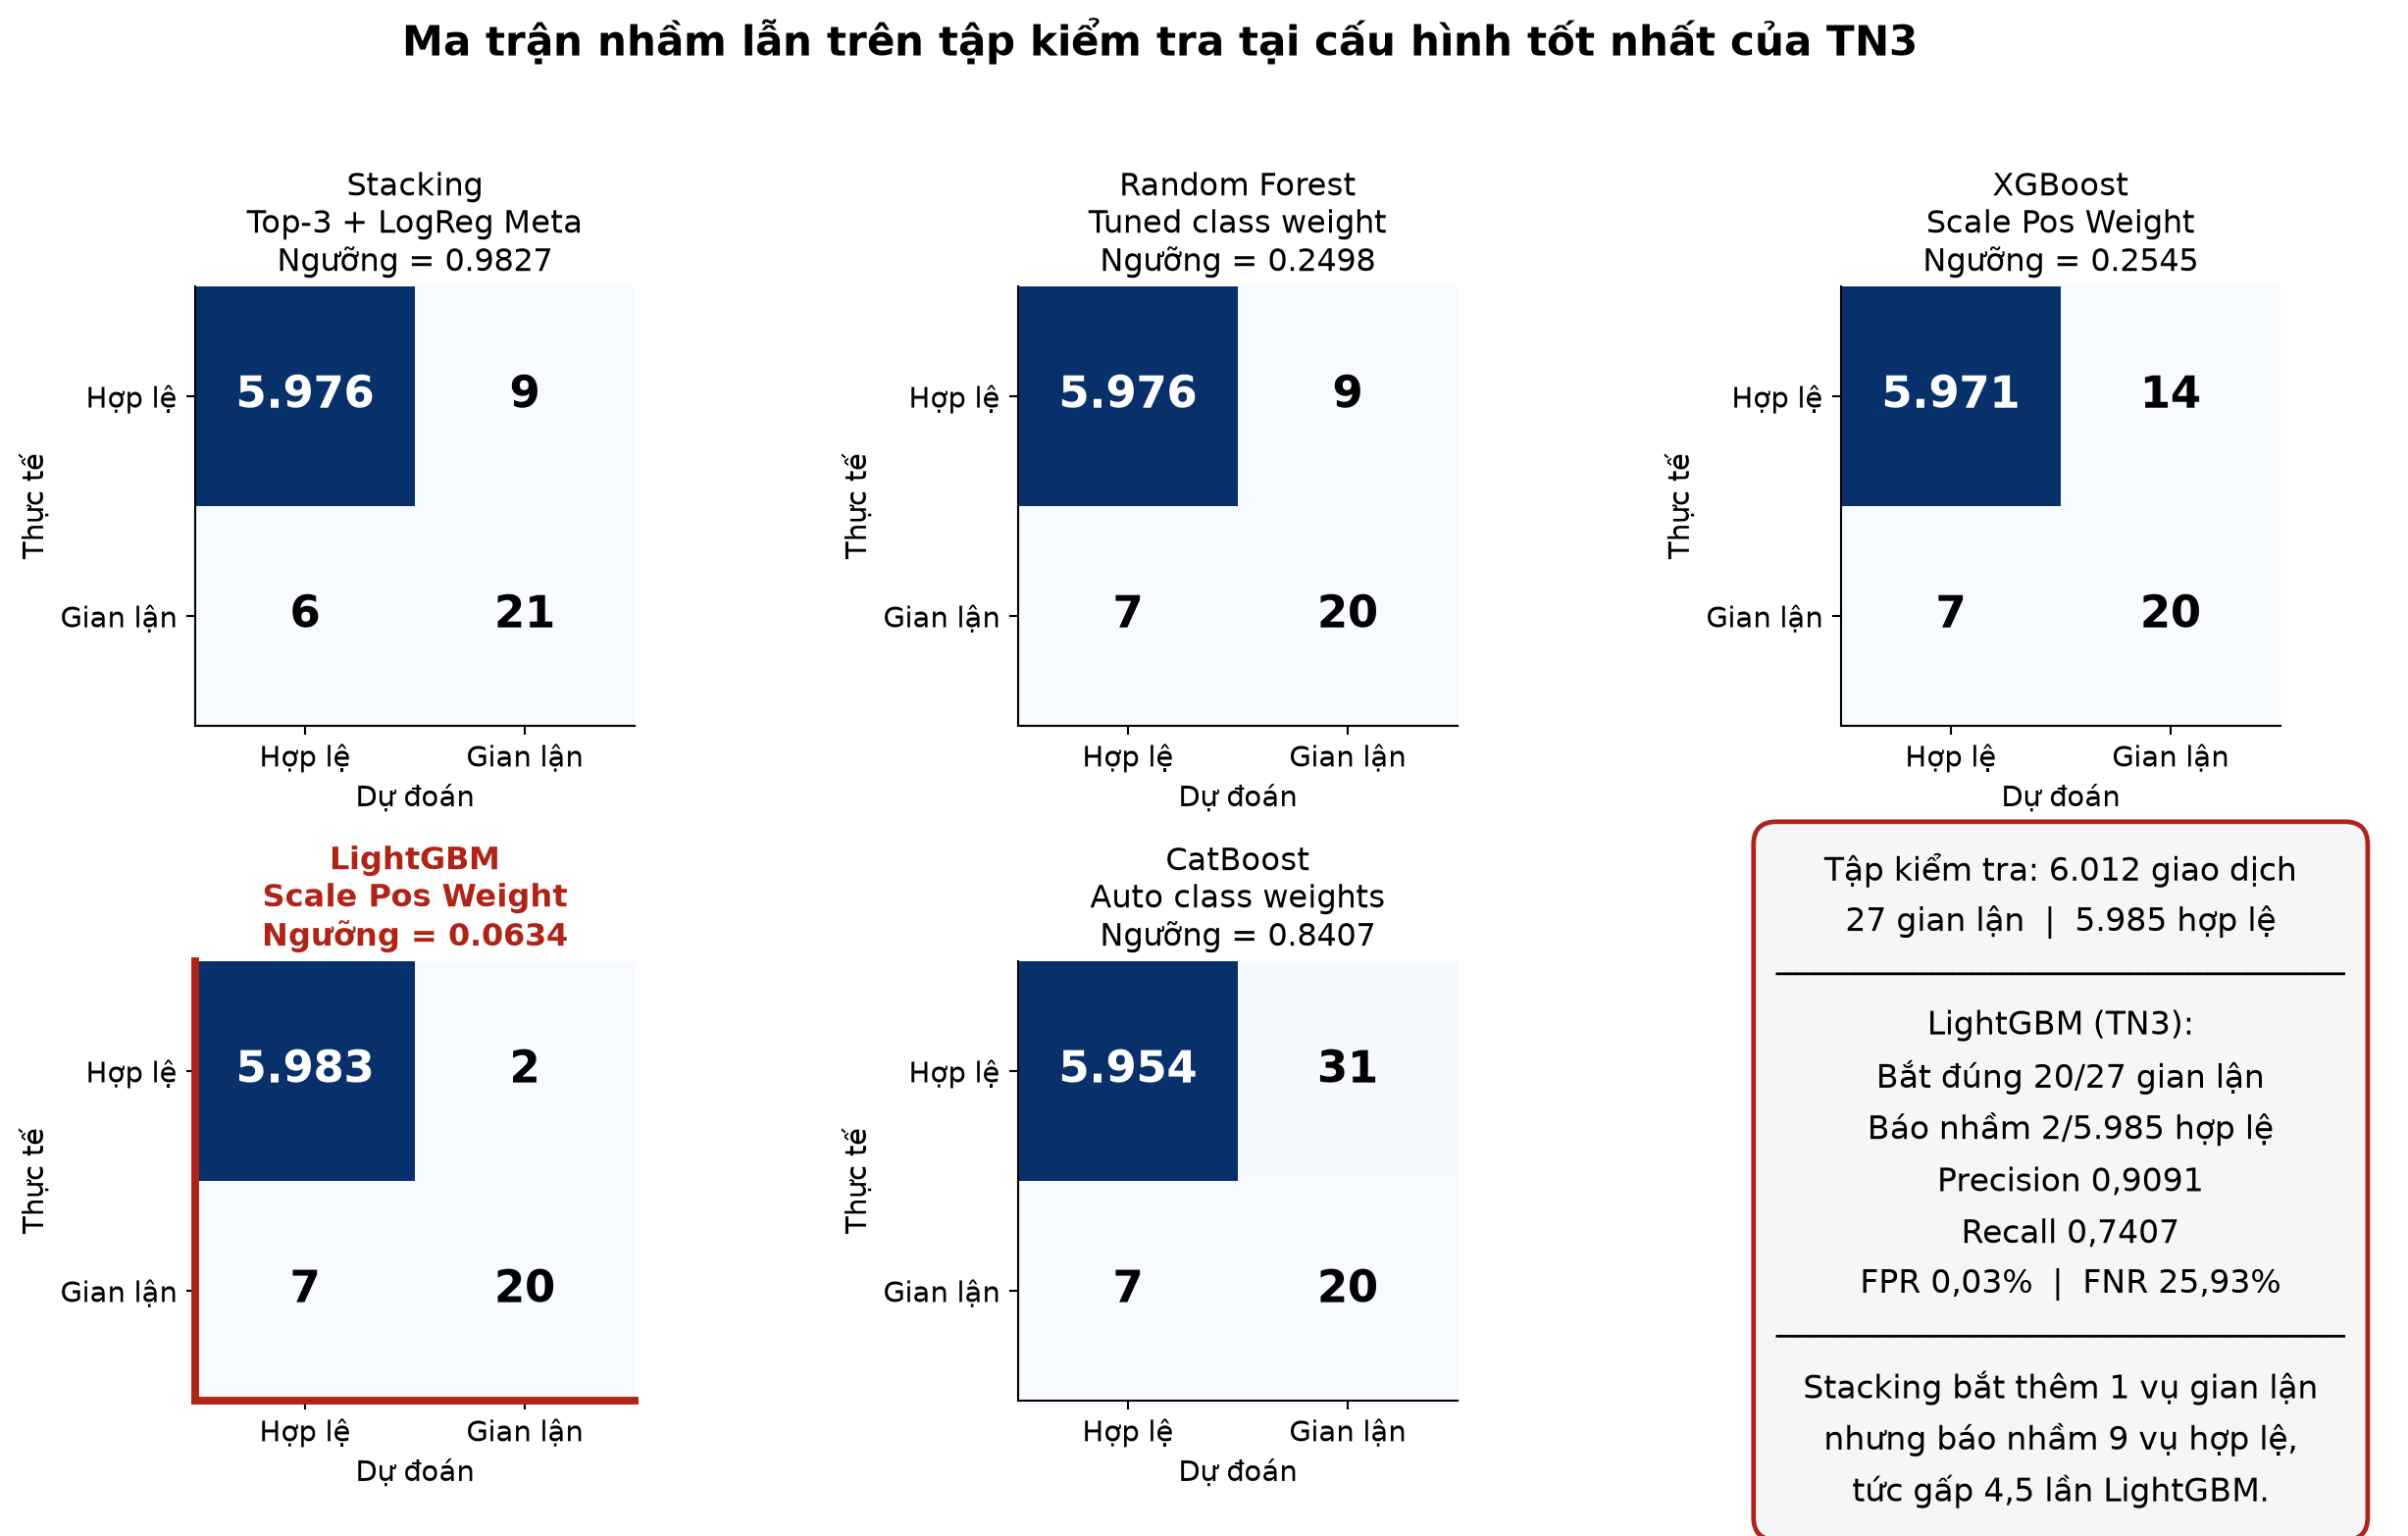
\includegraphics[width=\linewidth]{figures/fig_confusion_matrix.png}
    \caption{Ma trận nhầm lẫn của các mô hình tại cấu hình tốt nhất của thử nghiệm3 trên tập kiểm tra}
    \label{fig:confusion_matrix}
\end{figure}

Hình \ref{fig:confusion_matrix} trình bày ma trận nhầm lẫn của năm mô hình tại cấu hình tốt nhất của thử nghiệm3 trên tập kiểm tra. LightGBM phát hiện đúng 20 trong 27 giao dịch gian lận, bỏ sót 7, đồng thời chỉ báo nhầm 2 giao dịch hợp lệ --- con số thấp nhất trong năm mô hình. Stacking bắt được 21 trong 27 vụ, nhiều hơn đúng 1 vụ, nhưng phải chấp nhận 9 giao dịch hợp lệ bị báo nhầm, tức gấp 4{.}5 lần so với LightGBM; xét cả hai loại rủi ro thì Stacking không tốt bằng LightGBM. Ba mô hình còn lại cùng bắt 20 vụ nhưng báo nhầm lần lượt 9, 14 và 31 giao dịch hợp lệ. Xét theo tỷ lệ, FPR của LightGBM là 0{.}03\% trên 5\,985 giao dịch hợp lệ, tức thấp hơn tỷ lệ gian lận quan sát được là 0{.}45\%.

\begin{figure}[H]
    \centering
    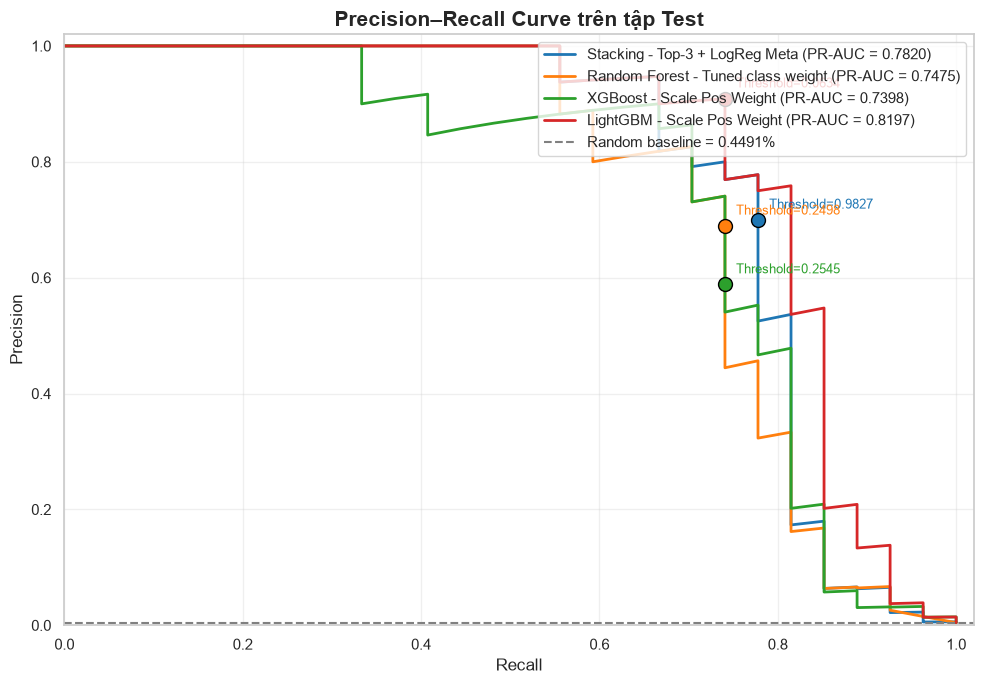
\includegraphics[width=0.9\linewidth]{figures/fig_pr_curve.png}
    \caption{Đường Precision--Recall của các mô hình tại cấu hình tốt nhất của thử nghiệm3 trên tập kiểm tra}
    \label{fig:pr_curve}
\end{figure}


\begin{figure}[H]
	\centering
	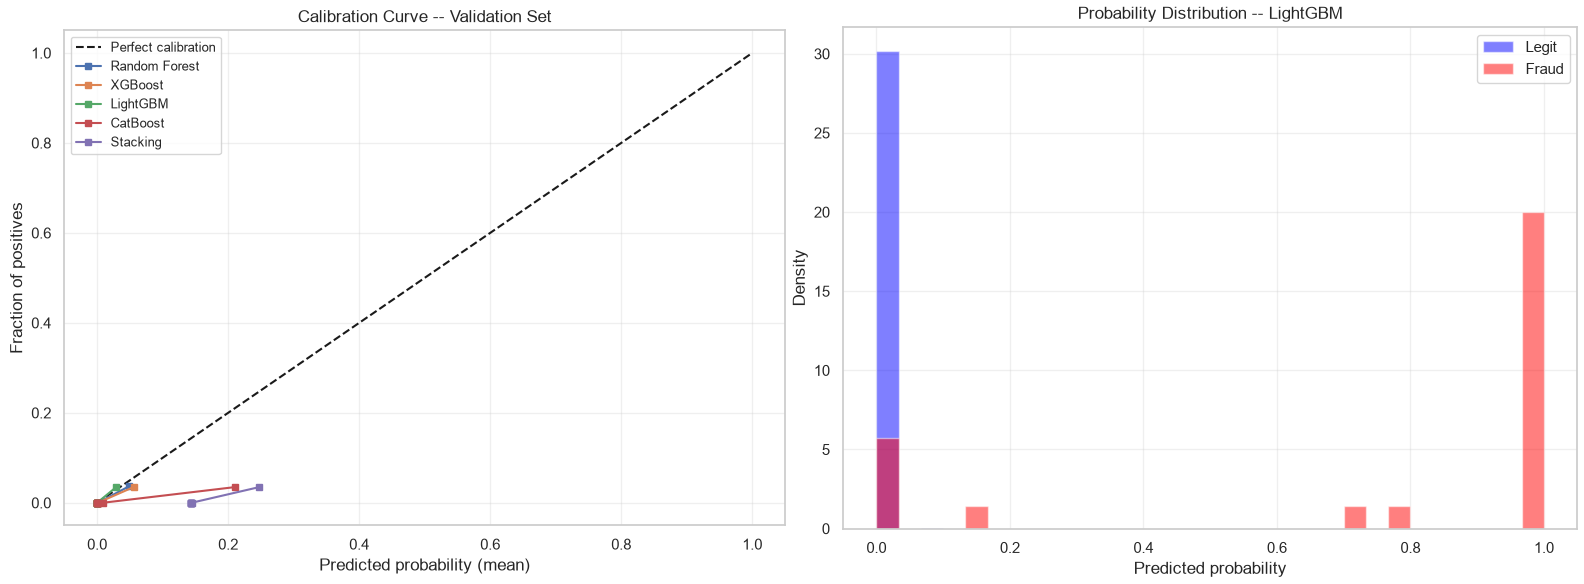
\includegraphics[width=\linewidth]{figures/fig_calibration_lightgbm.png}
	\caption{Đường hiệu chuẩn trên tập Validation và phân phối xác suất của mô hình LightGBM}
	\label{fig:calibration}
\end{figure}

Hình \ref{fig:pr_curve} vẽ đường Precision--Recall của bốn mô hình trên tập kiểm tra. Đường của LightGBM nằm cao hơn các đường còn lại trên hầu hết lân vùng thao tác thực tế, đạt PR-AUC 0{.}8197, tiếp theo là Stacking 0{.}7820, Random Forest 0{.}7475 và XGBoost 0{.}7398. Điểm hoạt động của LightGBM tại ngưỡng 0{.}0634 nằm ở vùng Recall cao với Precision 0{.}9091, tức độ chính xác cao gấp khoảng 202 lần so với dự đoán ngẫu nhiên. Đường nét đứt ngang là đường cơ sở ứng với tỷ lệ gian lận trong tập kiểm tra là 0{.}4491\%; toàn bộ các mô hình nằm trên đường này ở vùng ngưỡng đã chọn, xác nhận mô hình có giá trị thực tế.


Hình \ref{fig:calibration} bổ sung hai góc nhìn về chất lượng xác suất dự đoán. Đường hiệu chuẩn trên tập Validation cho thấy xác suất dự đoán của các mô hình thấp hơn đáng kể so với tần suất thực tế, một hạn chế chung của mô hình trên dữ liệu cực mất cân bằng. Biểu đồ phân phối xác suất của mô hình LightGBM cho thấy hai lớp tách biệt khá rõ: gần như toàn bộ giao dịch hợp lệ (99{.}94\%) tập trung ở vùng xác suất dưới 0{.}1, còn giao dịch gian lận tập trung ở vùng trên 0{.}8, với trung vị 0{.}997.

\section{Lựa chọn mô hình phù hợp với bộ dữ liệu}
Dựa trên sáu thử nghiệm, đề tài chọn LightGBM với \texttt{scale\_pos\_weight} trên tập 14 đặc trưng của thử nghiệm3 làm mô hình đề xuất cuối cùng. Lý do chọn được tóm tắt như sau:

\begin{itemize}
    \item Cân bằng tốt nhất trên ba chỉ số chính. LightGBM tại thử nghiệm3 đồng thời đạt F1-Score cao nhất (0{.}8163) và F2-Score cao nhất (0{.}7692) trong toàn bộ sáu thử nghiệm, với PR-AUC 0{.}8197 thuộc nhóm cao nhất. Như Bảng \ref{tab:exp_summary} cho thấy, không mô hình nào khác đạt đồng thời hai chỉ số F1 và F2 ở mức cao.
    \item Chi phí nghiệp vụ thấp nhất. Với Precision 0{.}9091, trong 22 giao dịch được cảnh báo có 20 là gian lận thật, tức chỉ 2 giao dịch hợp lệ bị kiểm tra lại không cần thiết --- tương đương FPR 0{.}0003. Đây là mức thấp nhất trong năm mô hình tại thử nghiệm3 và thấp hơn Stacking tới 5 lần (0{.}0015). Trong hệ thống thực tế, mỗi giao dịch hợp lệ bị chặn nhầm đều sinh chi phí xác minh và khiếu nại, nên đây là ưu thế quan trọng.
    \item Chi phí tính toán thấp. Thời gian dự đoán toàn bộ 6\,012 giao dịch là 0{.}0361 giây, nhanh nhất trong sáu thử nghiệm và thấp hơn thử nghiệm4 tới 2{.}9 lần; thời gian tinh chỉnh siêu tham số là 231{.}85 giây, giảm 4{.}9 lần so với thử nghiệm2 và 9{.}6 lần so với thử nghiệm4.
    \item Không đánh đổi nhiều Recall để lấy PR-AUC. thử nghiệm4 có PR-AUC cao hơn 0{.}0034 nhưng F2-Score thấp hơn 0{.}0058, FPR cao hơn và thời gian dự đoán gấp 2{.}9 lần. Với chỉ 27 mẫu gian lận trong tập kiểm tra, chênh lệch 0{.}0034 tương đương dưới 0{.}1\% và nằm trong biên sai số, không đủ căn cứ để đánh đổi.
\end{itemize}

Về hướng cải thiện Recall, vì bản chất nghiệp vụ ưu tiên bắt gian lận hơn là giảm báo nhầm, nếu hệ thống cần Recall cao hơn thì nên hạ ngưỡng quyết định của LightGBM xuống dưới 0{.}0634 thay vì đổi sang mô hình khác: theo đường Precision--Recall tại Hình \ref{fig:pr_curve}, hạ ngưỡng làm Recall tăng nhanh hơn đáng kể so với đổi mô hình, trong khi Precision giảm chậm. Ngưỡng vận hành cụ thể nên được chọn theo chi phí tương đối giữa một vụ gian lận bị bỏ sót và một giao dịch hợp lệ bị chặn nhầm, thay vì cố định theo F2-Score.

\section{Đánh giá tính khả thi và hạn chế}
\subsection{Điểm mạnh}
\begin{itemize}
    \item Quy trình hoàn chỉnh từ nạp dữ liệu, làm sạch, tạo đặc trưng đến huấn luyện và đánh giá, sát với bài toán phân loại nhị phân mất cân bằng trong thực tế.
    \item Thiết kế sáu thử nghiệm có kiểm soát: ba thử nghiệm tách ảnh hưởng của phương pháp mã hóa, ba thử nghiệm còn lại kiểm tra ảnh hưởng của việc loại bỏ đặc trưng, nhờ đó kết luận về tầm quan trọng của kỹ thuật tạo đặc trưng và của \texttt{TargetEncoder} có cơ sở thực nghiệm thay vì chỉ dựa trên kinh nghiệm.
    \item Khảo sát đồng thời bốn họ thuật toán rừng ngẫu nhiên và gradient boosting (XGBoost, LightGBM, CatBoost) cùng bốn chiến lược xử lý mất cân bằng khác nhau, đồng thời kết hợp các mô hình tốt nhất bằng stacking, bảo đảm khách quan khi so sánh hiệu quả.
    \item Thiết kế quy trình đánh giá nghiêm ngặt: tách riêng tập Fit, Validation và tập kiểm tra; giới hạn giá trị bất thường và chuẩn hóa chỉ học từ tập huấn luyện, giúp tránh rò rỉ dữ liệu.
    \item Sử dụng bộ chỉ số phù hợp với dữ liệu mất cân bằng gồm F2-Score và PR-AUC thay vì Accuracy, kèm báo cáo riêng FNR và FPR để phản ánh trực tiếp hai loại rủi ro của hệ thống.
\end{itemize}

\subsection{Hạn chế}
\begin{itemize}
    \item Bộ dữ liệu là dữ liệu mô phỏng với thời gian quan sát ngắn 10 ngày, chưa phản ánh đầy đủ các phương thức gian lận mới phát sinh theo thời gian.
    \item Tập kiểm tra chỉ chứa 27 giao dịch gian lận, nên mỗi giao dịch đúng thay đổi Recall khoảng 0{.}037. Chênh lệch PR-AUC giữa thử nghiệm3 và thử nghiệm4 là 0{.}0034, nhỏ hơn nhiều lần sai số này, khiến việc phân định thứ hạng giữa hai cấu hình chưa thật sự chắc chắn.
    \item Đặc trưng khoảng cách \texttt{distance\_km} tạo ra từ vị trí địa lý chứa nhiễu do chất lượng dữ liệu tọa độ, có thể làm giảm hiệu quả của mô hình.
    \item Xác suất dự đoán của các mô hình chưa được hiệu chuẩn tốt trên tập Validation, ảnh hưởng đến việc diễn giải ngưỡng quyết định theo xác suất tuyệt đối.
    \item Các khoảng siêu tham số được khảo sát bằng tìm kiếm ngẫu nhiên với số lần thử có giới hạn, chưa khẳng định được cấu hình tối ưu toàn cục.
\end{itemize}

\section{Hướng phát triển trong tương lai}
\begin{itemize}
    \item Mở rộng dữ liệu thực tế nhiều tháng và bổ sung các đặc trưng như dấu vân tay thiết bị, địa chỉ IP, lịch sử tranh chấp của thẻ.
    \item Thử thêm các tổ hợp loại bỏ đặc trưng khác, so sánh \texttt{TargetEncoder} với \texttt{CatBoostEncoder} và mã hóa theo chuỗi thời gian, nhằm cải thiện thêm Recall.
    \item Hiệu chuẩn xác suất dự đoán bằng \texttt{CalibratedClassifierCV} và chọn ngưỡng vận hành theo chi phí kinh doanh thay vì chỉ theo F2-Score.
    \item Áp dụng các kỹ thuật nâng cao như điều chỉnh trọng số lớp theo chi phí nghiệp vụ, học sâu trên chuỗi giao dịch, hoặc tinh chỉnh siêu tham số có hệ thống bằng tối ưu hóa Bayes.
    \item Mở rộng stacking với nhiều mô hình cơ sở và bộ tổng hợp khác nhau.
    \item Triển khai hệ thống chấm điểm theo thời gian thực với giám sát độ trễ và phát hiện lệch phân bố dữ liệu sau khi đưa vào vận hành.
\end{itemize}


\chapter{KẾT LUẬN}
Trong khuôn khổ môn học Trí tuệ nhân tạo, đề tài đã xây dựng một quy trình hoàn chỉnh để phát hiện giao dịch thẻ tín dụng bất thường và nghi vấn gian lận, từ khâu nạp, làm sạch dữ liệu đến khâu thiết kế thử nghiệm, huấn luyện và đánh giá mô hình. Bộ dữ liệu gồm 30\,058 giao dịch trong giai đoạn 21/06--30/06/2020, trong đó 133 giao dịch gian lận, chiếm 0{,}44\%. Phân tích khám phá cho thấy gian lận tập trung ở vài loại dịch vụ (\texttt{shopping\_net}, \texttt{misc\_net}, \texttt{grocery\_pos} chiếm 82/133 vụ) và 104/133 vụ nằm trong vùng số tiền bất thường.

Đề tài xây dựng 14 đặc trưng, huấn luyện bốn họ thuật toán (Random Forest, XGBoost, LightGBM, CatBoost) với bốn chiến lược cân bằng mất cân bằng dữ liệu, kết hợp ba mô hình tốt nhất bằng stacking, chọn ngưỡng theo F2-Score trên tập Validation và đánh giá một lần duy nhất trên tập kiểm tra gồm 6\,012 giao dịch có 27 giao dịch gian lận.

Kết quả cho thấy kỹ thuật tạo đặc trưng đóng vai trò quyết định: với sáu đặc trưng gốc, PR-AUC chỉ đạt 0{,}5016, còn khi bổ sung nhóm đặc trưng kỹ thuật và mã hóa bằng \texttt{TargetEncoder} thì đạt 0{,}8197. So với \texttt{OneHotEncoder}, \texttt{TargetEncoder} vừa nâng cao hiệu quả vừa giảm số chiều từ 26 xuống 14 và rút ngắn thời gian tinh chỉnh còn 232 giây; ba thử nghiệm loại bỏ đặc trưng đều không làm mô hình tốt hơn. Xét tổng thể, LightGBM là thuật toán bền vững nhất: dẫn đầu PR-AUC ở cả năm thử nghiệm có nó và giữ FPR ở mức 0{,}0003--0{,}0017, còn các thuật toán khác biến động mạnh theo tập đặc trưng.

Vì vậy, đề tài chọn LightGBM với \texttt{scale\_pos\_weight} trên 14 đặc trưng mã hóa bằng \texttt{TargetEncoder} (thử nghiệm 3) làm mô hình đề xuất. Mô hình đạt PR-AUC 0{,}8197, F1-Score 0{,}8163 và F2-Score 0{,}7692 --- đều cao nhất trong sáu thử nghiệm --- với Precision 0{,}9091, Recall 0{,}7407; thời gian dự đoán toàn bộ 6\,012 giao dịch chỉ 0{,}036 giây.

Đề tài còn hạn chế do dữ liệu mô phỏng chỉ quan sát trong 10 ngày, số mẫu gian lận nhỏ, đặc trưng khoảng cách nhiễu tọa độ và xác suất dự đoán chưa hiệu chuẩn. Hướng phát triển là mở rộng dữ liệu thực tế, bổ sung đặc trưng hành vi thiết bị, hiệu chuẩn xác suất và chọn ngưỡng theo chi phí kinh doanh, rồi giám sát giao dịch. Tóm lại, đề tài đã minh họa quy trình phát hiện gian lận tài chính bằng trí tuệ nhân tạo và cung cấp cơ sở so sánh về hiệu quả các thuật toán. Với 80\% giao dịch hợp lệ không bị chặn nhầm và thời gian dự đoán dưới 0{,}04 giây, mô hình đề xuất đủ để thử nghiệm trong hệ thống chấm điểm rủi ro thời gian thực.


\end{justify}
\end{spacing}

\printbibliography

\end{document}